\chapter{System Validation}\label{ch:validation}

This chapter presents the validation of the proposed solution.
The validation process is described in different sections, each addressing multiple components of the system.
Section~\ref{sec:meth} outlines the methodology used for validation.
Section ~\ref{sec:experimental-setup} presents the experimental setup.
Section ~\ref{sec:component-testing}, presents the individual testing of each system's component demonstrating its proper functioning.
Section~\ref{sec:use_case} describes a specific use case to demonstrate the system's functionality.
Finally, Section~\ref{sec:discuss} provides a discussion of the results and conclusions obtained from the validation process.

\section{Methodology}\label{sec:meth}
We have divided our tests into three categories: component testing, interoperability testing and use case validation.
The first category was used to validate the proper functioning of each component, including a performance evaluation.
The second category allowed us to determine if the components were working together properly.
The last category was defined to validate the proposed system in a reference scenario.
We conducted functional and performance validations using tools such as \emph{ping} and \emph{Iperf}~\cite{iperf}.

\section{Experimental Setup}\label{sec:experimental-setup}
This section presents the experimental setup.
Figure~\ref{fig:setup} depicts the experimental scenario considered.

\begin{figure}[H]
    \centering
    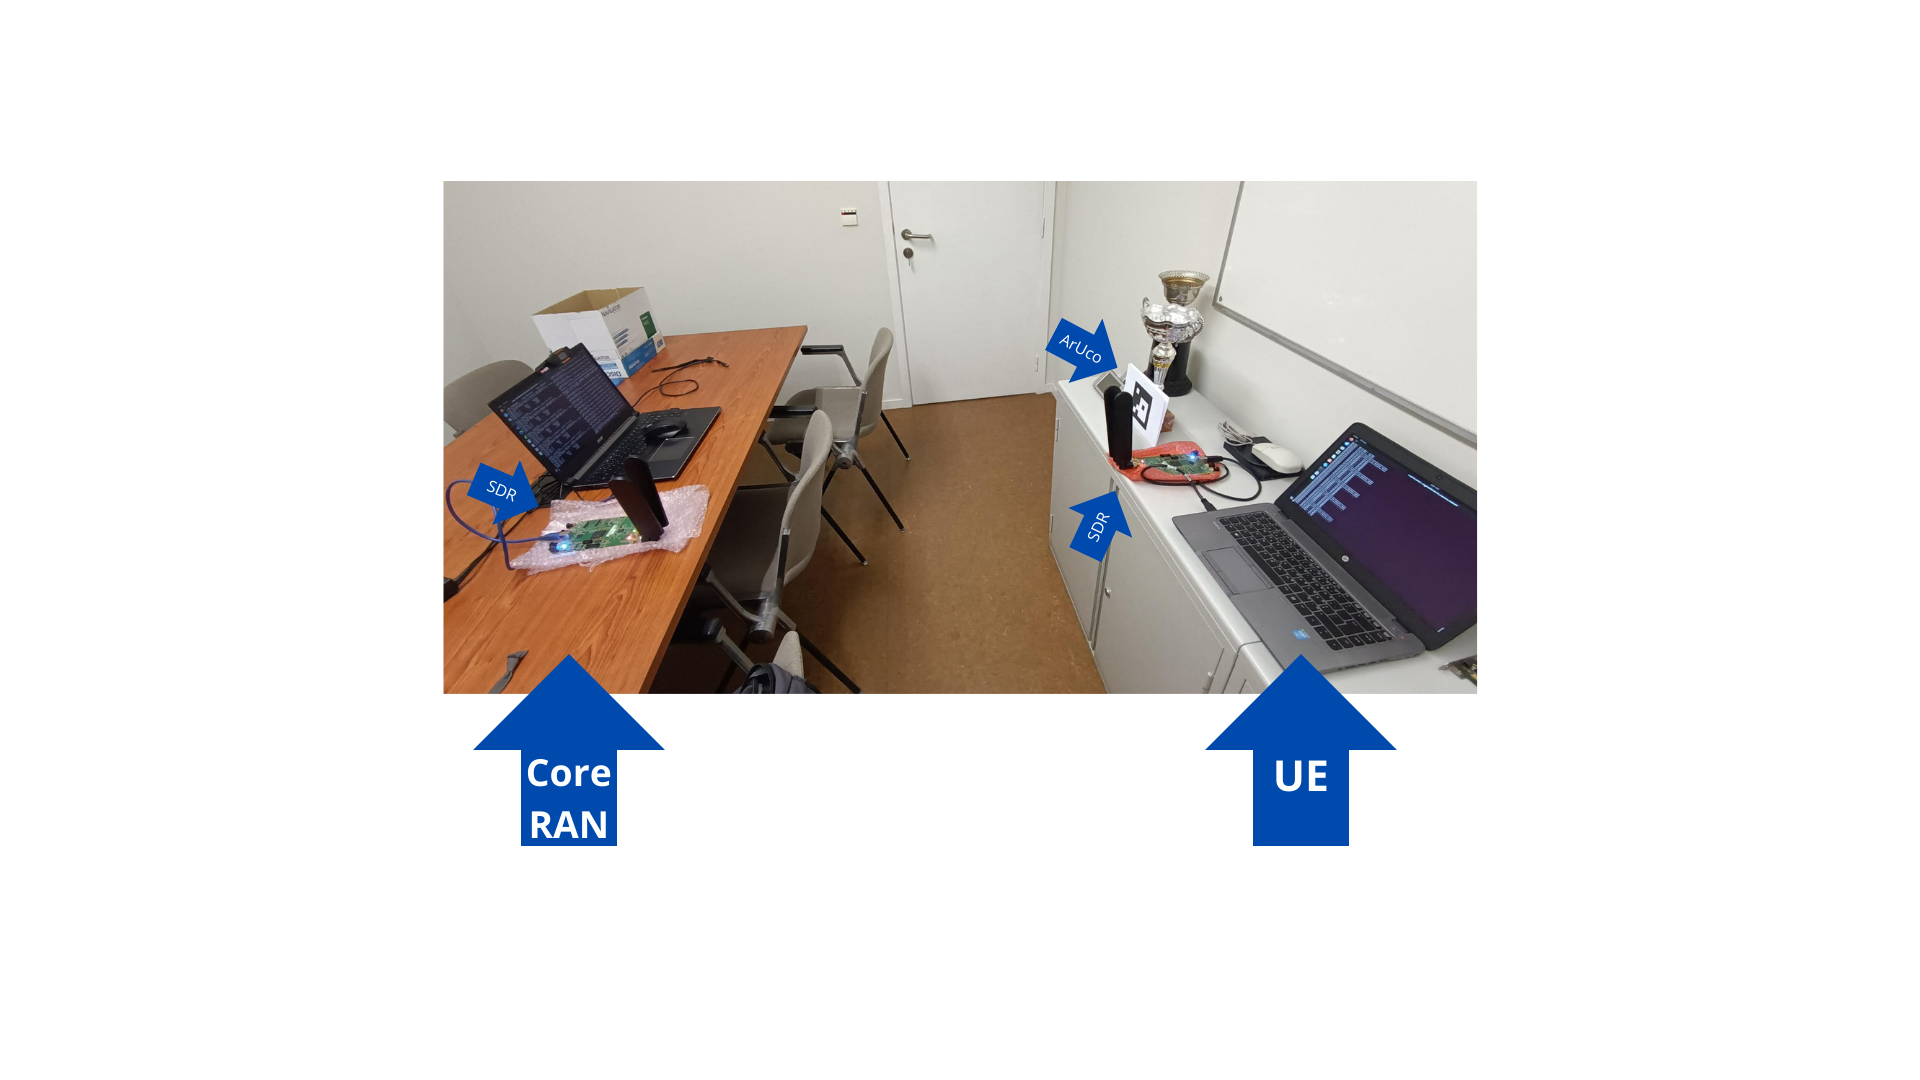
\includegraphics[width=\linewidth]{figures/setup}
    \caption{Experimental setup.}
    \label{fig:setup}
\end{figure}

Since we did not use a mmWave carrier frequency, in order to produce a greater attenuation introduced by an obstacle, we used an RF absorbing material.
The attenuation introduced by obstacles is not significant.
A person acting as the obstacle, holds the material when passing between the gNB and UE\@.
Figure~\ref{fig:foam} shows the RF absorbing material used.

\begin{figure}[H]
    \centering
    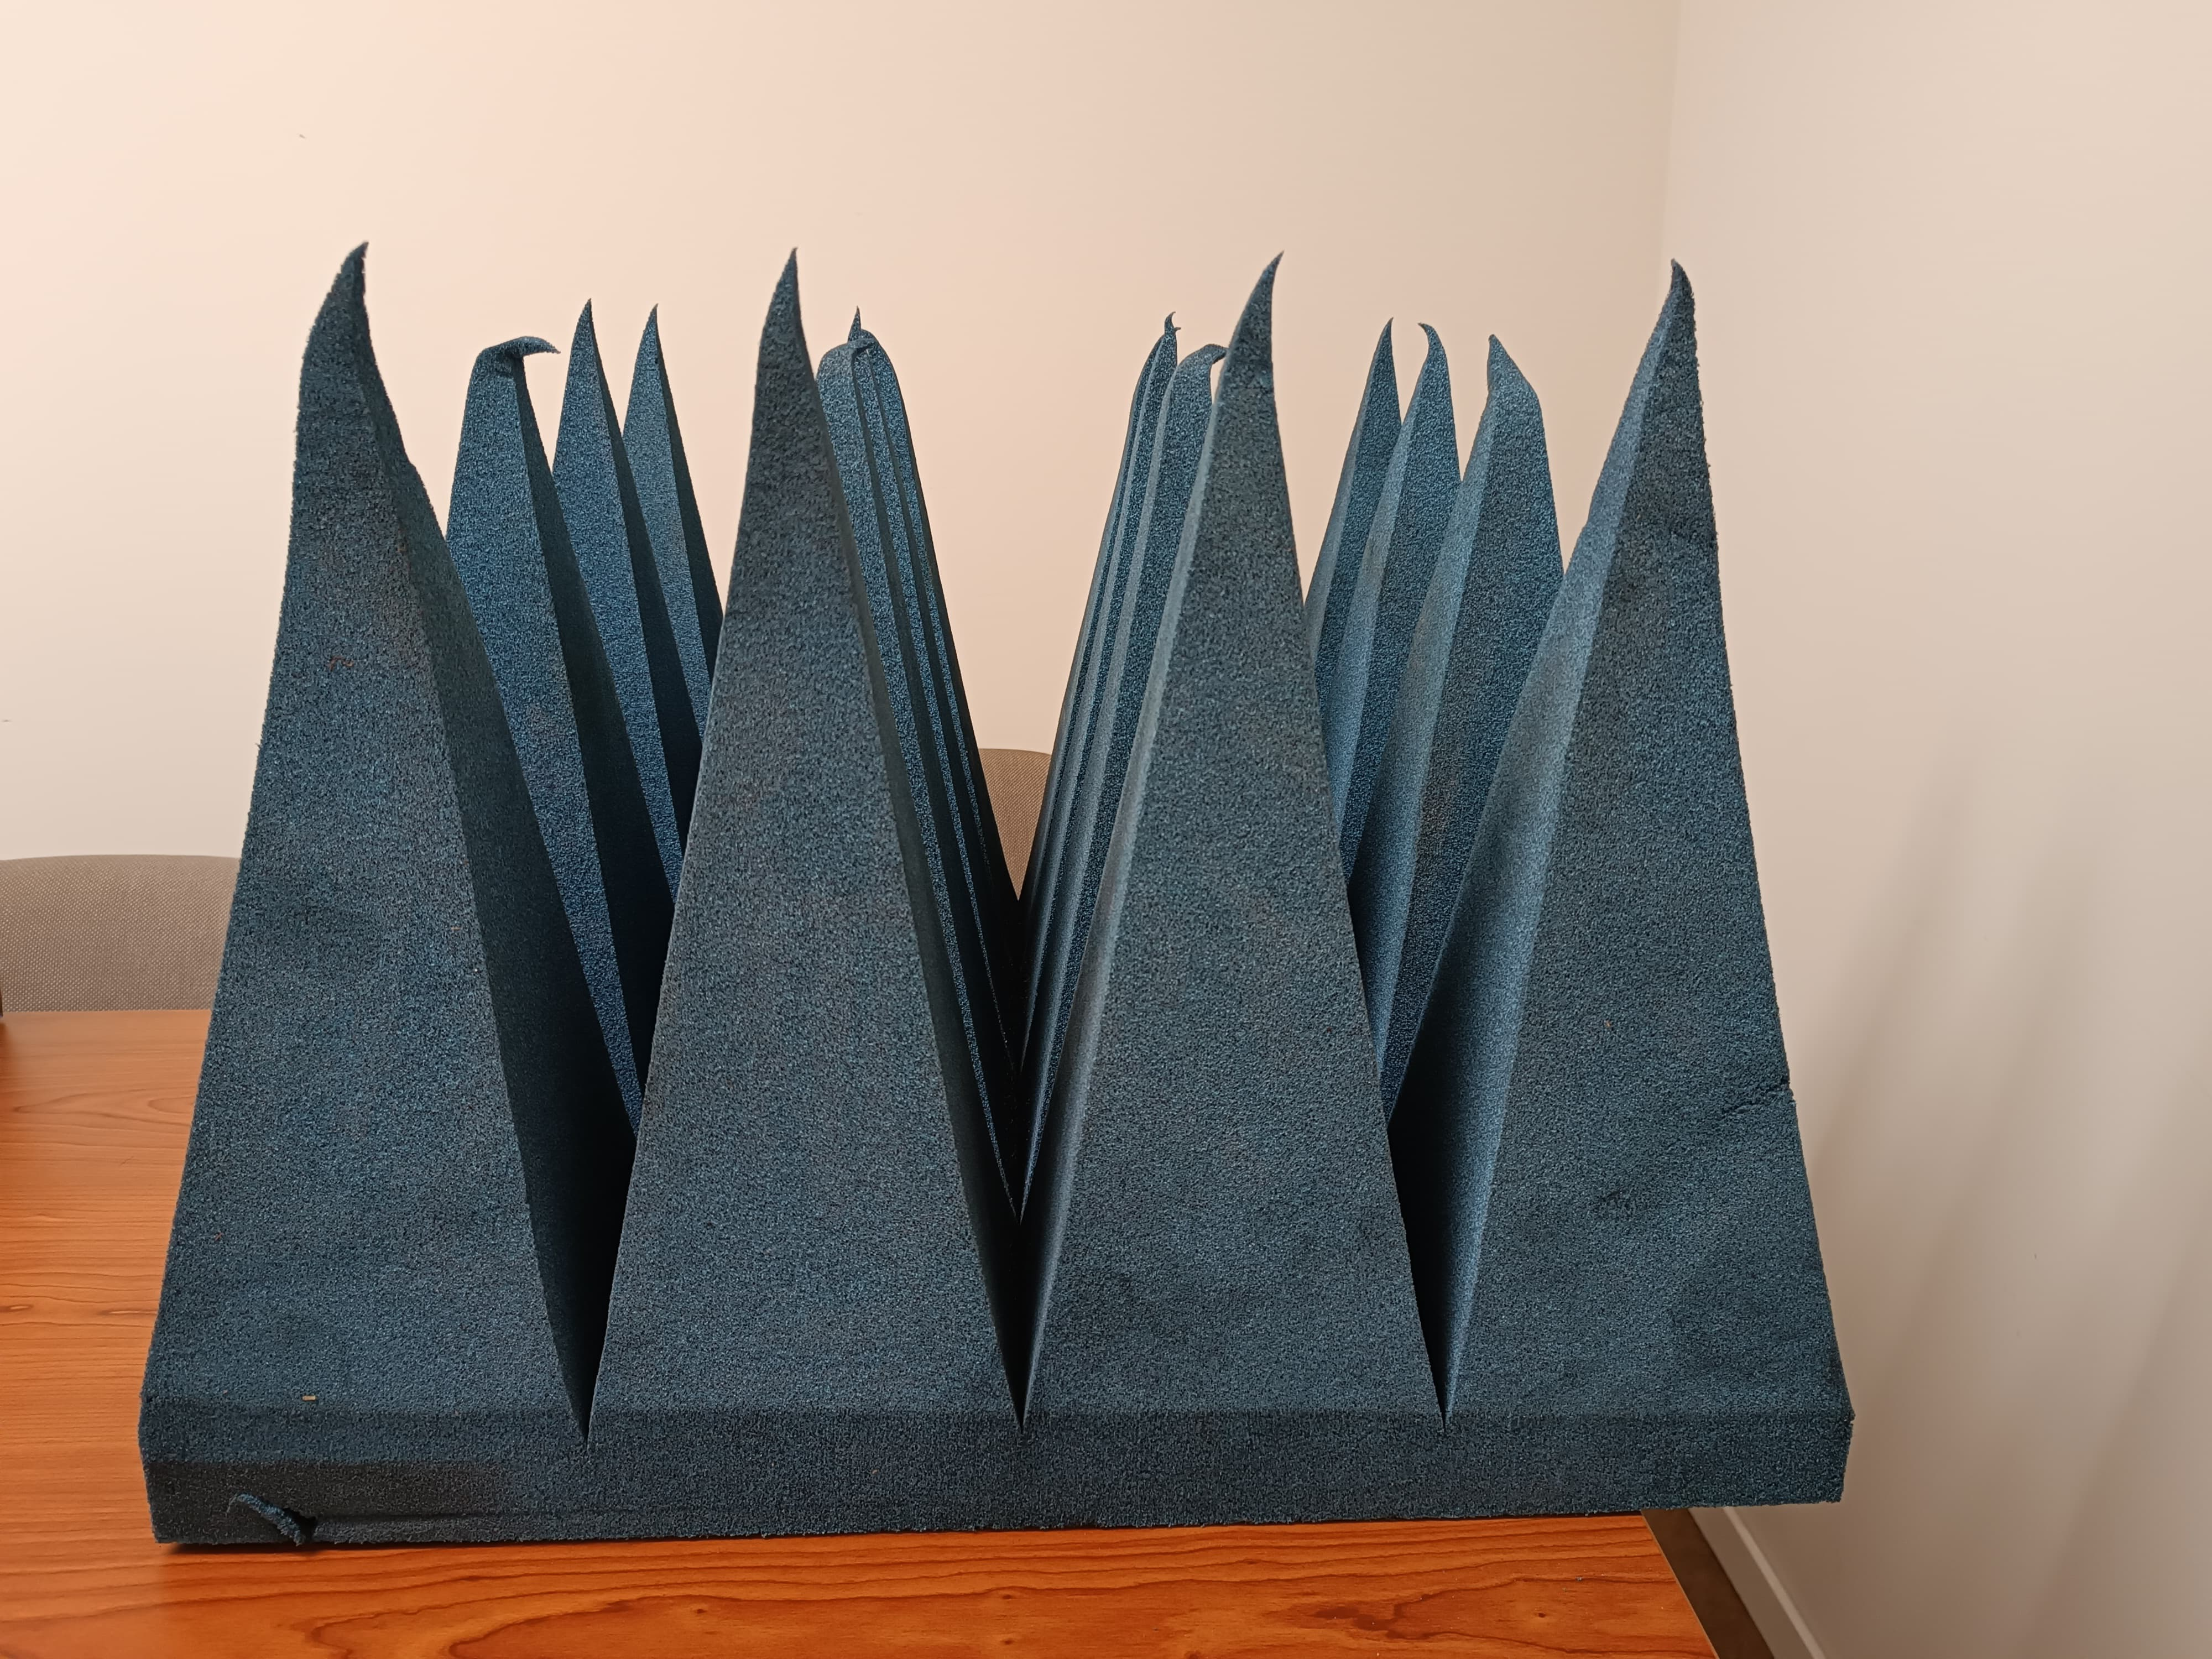
\includegraphics[width=0.5\linewidth]{figures/foam}
    \caption{Material used to absorve RF signals, in order to simulate strong attenuation introduced by obstacles.}
    \label{fig:foam}
\end{figure}



\section{Component and interoperability testing}\label{sec:component-testing}


\subsection{5G Core Network}\label{subsec:core_network}
In this section, the Core Network configuration and validation are discussed.
This includes the setup of network elements, their interactions, and performance metrics.
In order to ensure that all Core Network components were working properly, we performed a functional test.
The Core Network was deployed using Docker containers.
Figure~\ref{fig:core_init} shows the command for running the Core Network setup script.
After the Docker containers initialized, the setup script logs can be seen, indicating successful initialization.

\begin{figure}[H]
    \centering
    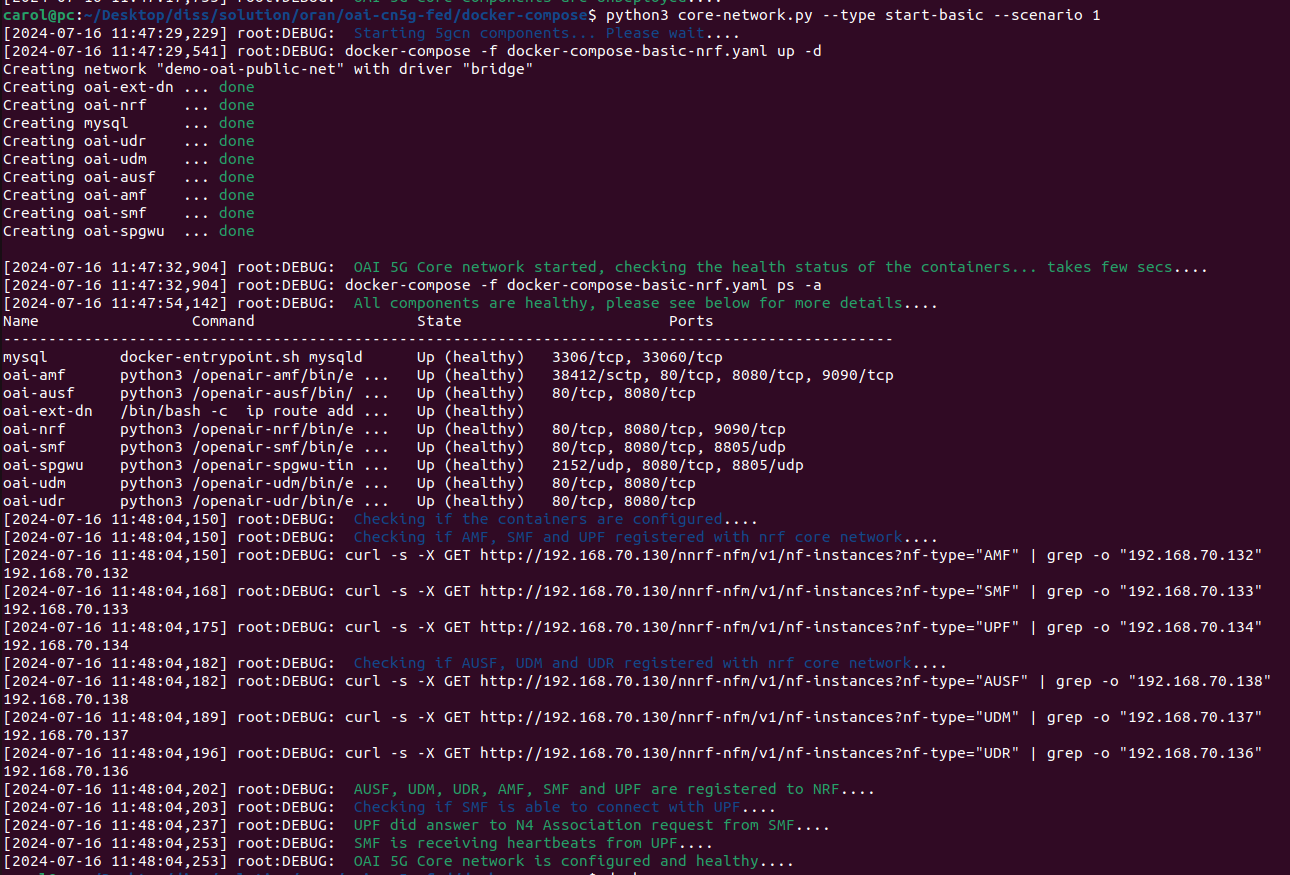
\includegraphics[width=0.7\linewidth]{figures/core_init}
    \caption[Initialization of the Core Network]{Initialization of the Core Network.}
    \label{fig:core_init}
\end{figure}

In order to confirm the correct deployment, the interface \textit{demo-oai} must appear when running the \textit{ifconfig} command.
Then, we verified that the containers had connectivity using the interface created in the Host OS, with the ping tool, as shown by Figure ~\ref{fig:ping_core1} and Figure~\ref{fig:ping_core2}.
Successfully concluding these tests ensured that the 5G Core Network was operational.

\begin{figure}[H]
\centering
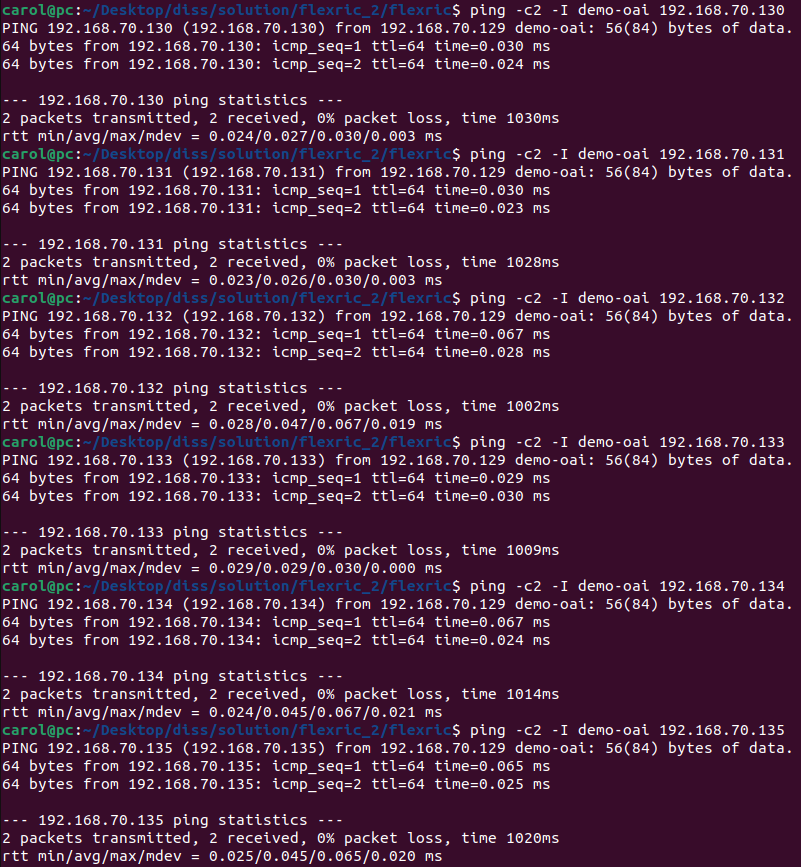
\includegraphics[width=0.5\linewidth]{figures/ping_core_1}
\caption[Pinging Core Network components from Host OS
interface]{Pinging Core Network components from Host OS
interface.}
\label{fig:ping_core1}
\end{figure}

\begin{figure}[H]
    \centering
    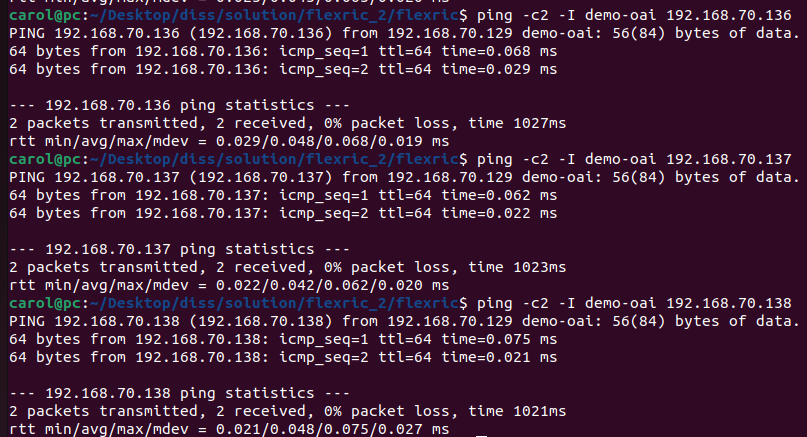
\includegraphics[width=0.5\linewidth]{figures/ping_core_2}
    \caption[Pinging Core Network components from Host OS
    interface]{Pinging Core Network components from Host OS
    interface.}
    \label{fig:ping_core2}
\end{figure}




\subsection{FlexRIC}\label{subsec:flexric2}
For the FlexRIC deployment, it was also necessary to ensure its correct launch.
Upon launching, it awaits incoming connection requests from an E2 Node.
Figure~\ref{fig:near-rt-ric} shows the initialization of FlexRIC\@.
When it is properly launched, the gNB can be initialized.

\begin{figure}[H]
    \centering
    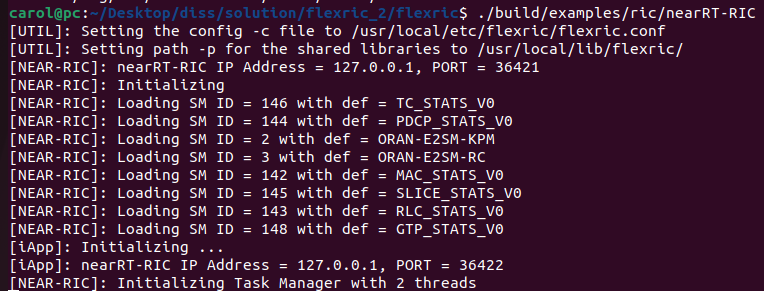
\includegraphics[width=0.7\linewidth]{figures/flexric_init}
    \caption{Initialization of FlexRIC's executable.}
    \label{fig:near-rt-ric}
\end{figure}

\subsection{gNB}\label{subsec:gnb}
To ensure the correct functioning of the gNB, it should be registered in the 5G Core Network, connected to the FlexRIC, and registered as an E2 node.
They need to be validated separately, as the connections are independent.

After executing the command to launch the gNB\@, the proper operation of the SDR can be verified by its Light-Emitting Diodes (LEDs).
Three LEDs  -- blue, red, and green -- indicate the powering of the SDR, the transmission, and the reception of radio signals, respectively, as depicted in Figure~\ref{fig:usrp_working}.

\begin{figure}[H]
    \centering
    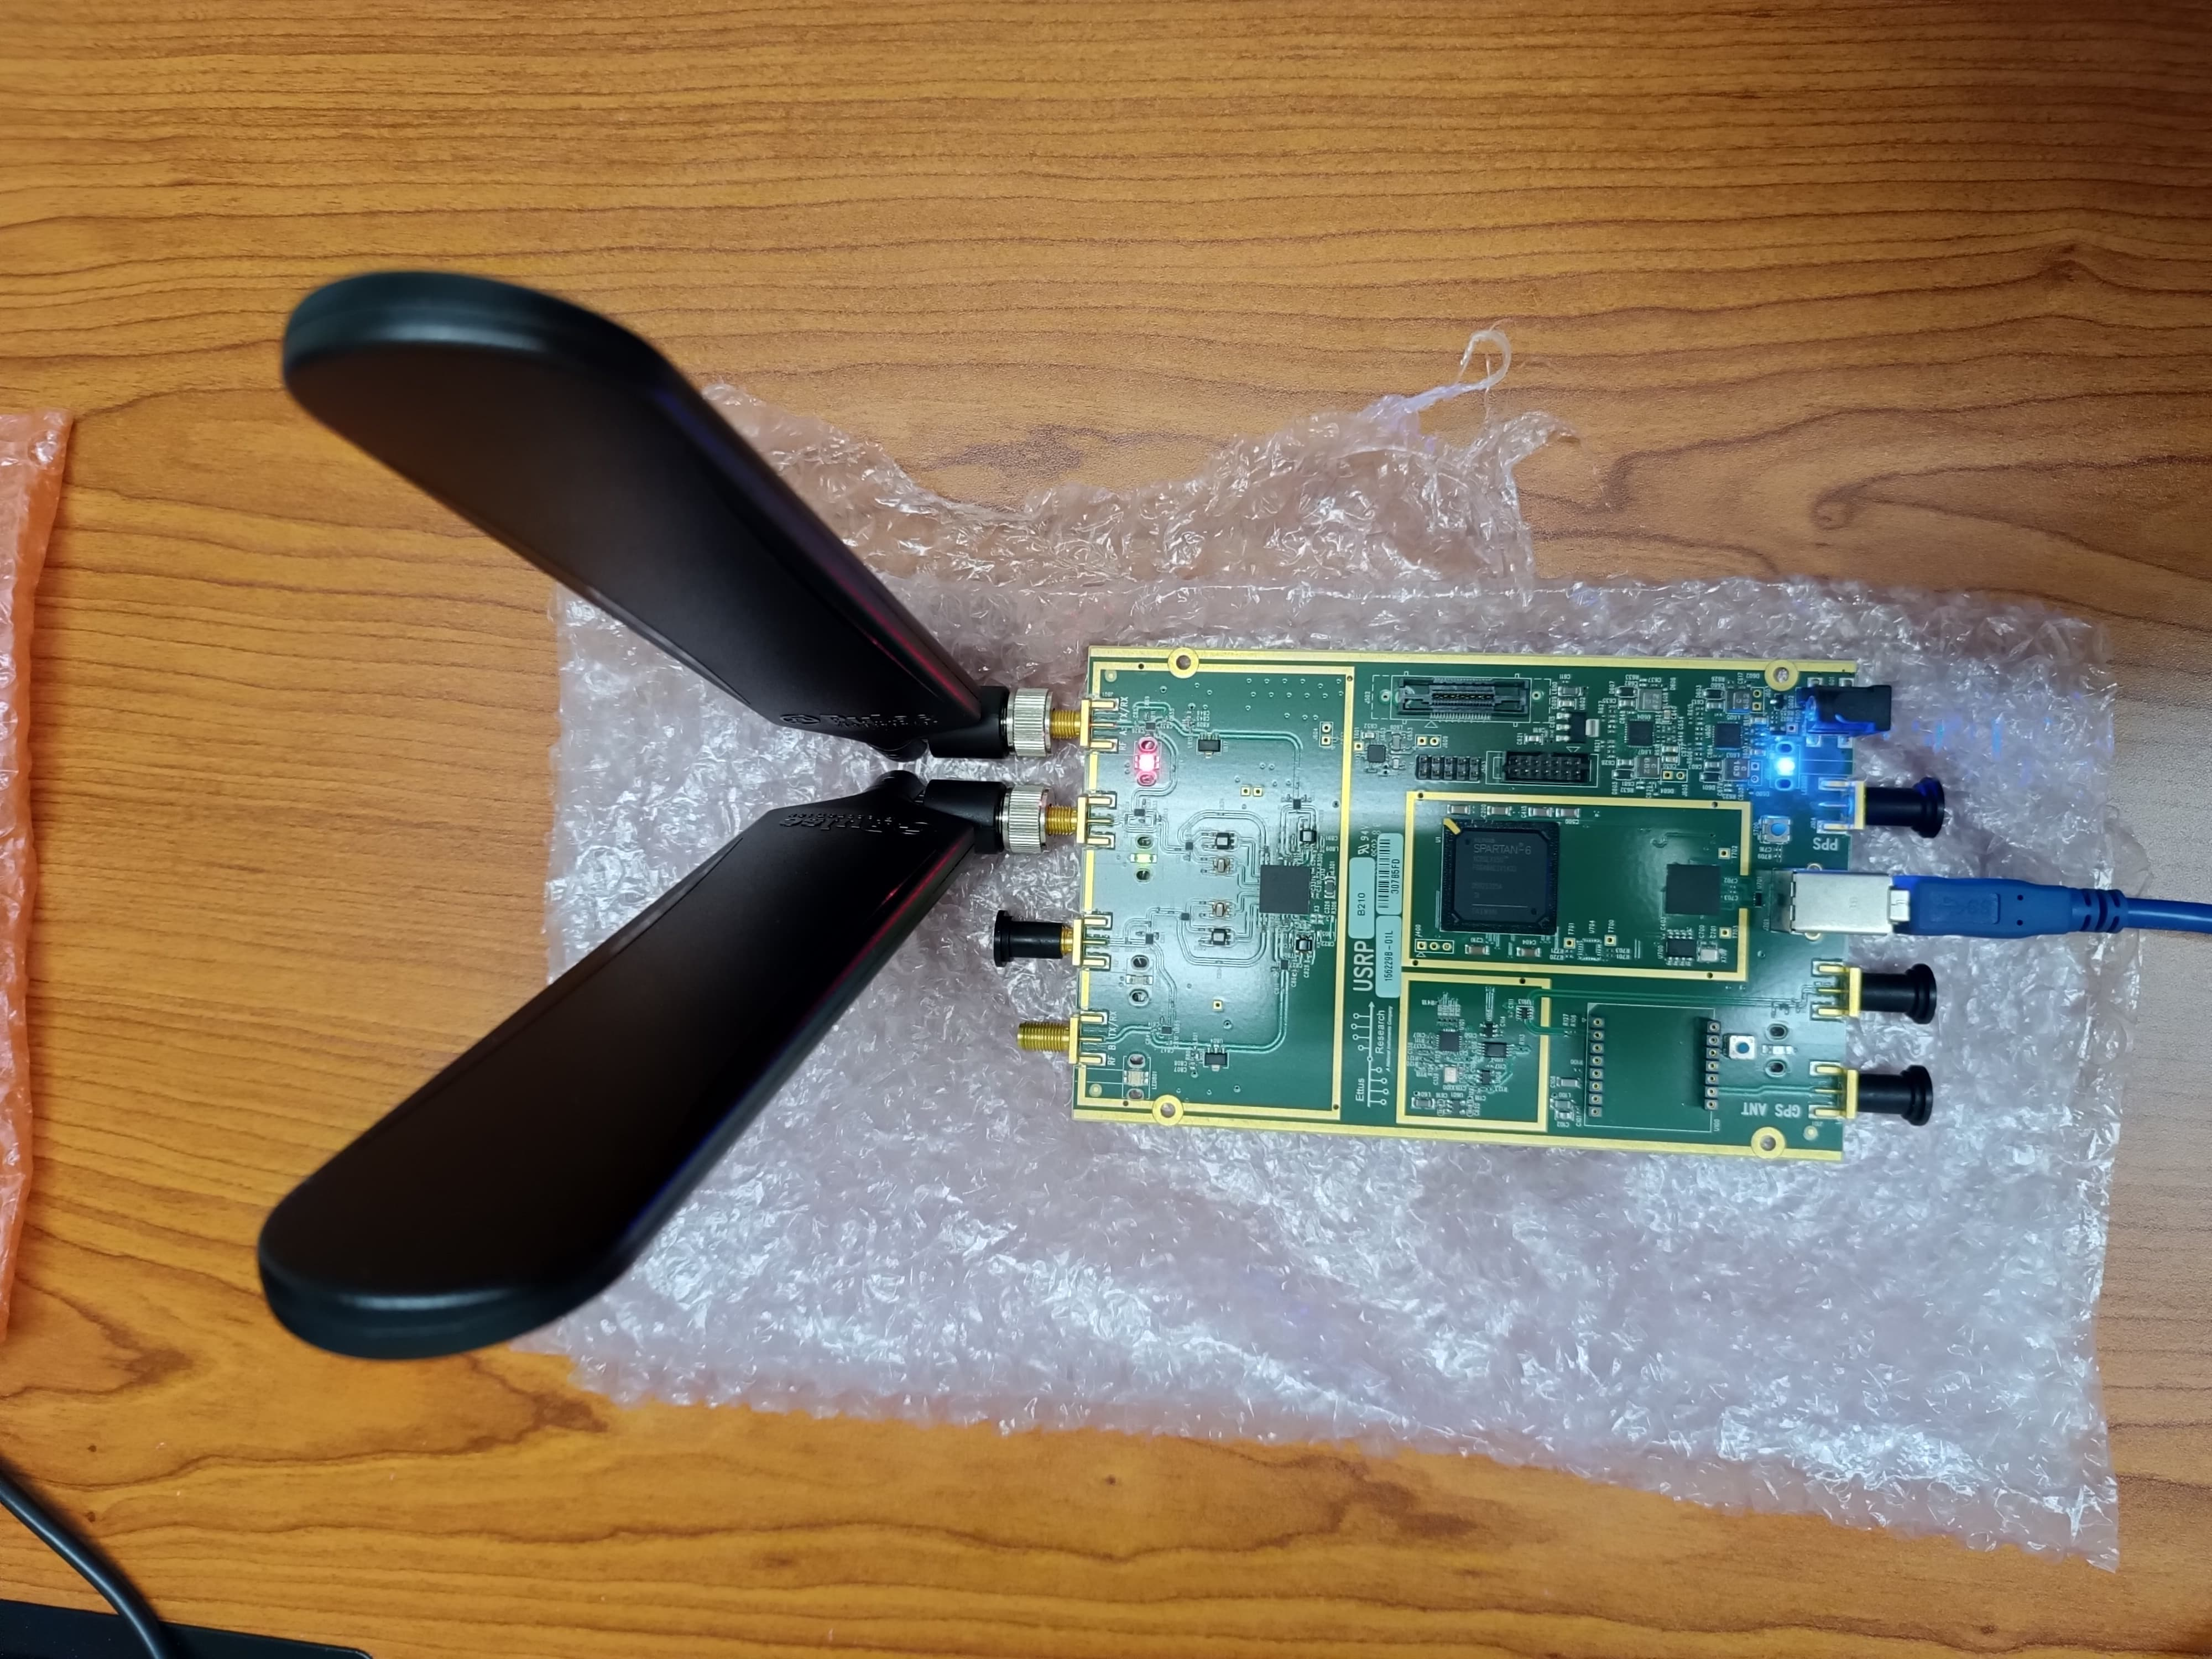
\includegraphics[width=0.5\linewidth]{figures/usrp_working}
    \caption[USRP B210 SDR operating]{USRP B210 SDR operating.}
    \label{fig:usrp_working}
\end{figure}

To ensure the correct registration in the Core Network, it was necessary to check the packet exchange between gNB and Core, using Wireshark.
Figure~\ref{fig:gnb_reg} shows the successful registration of the gNB with the AMF\@.

\begin{figure}[H]
    \centering
    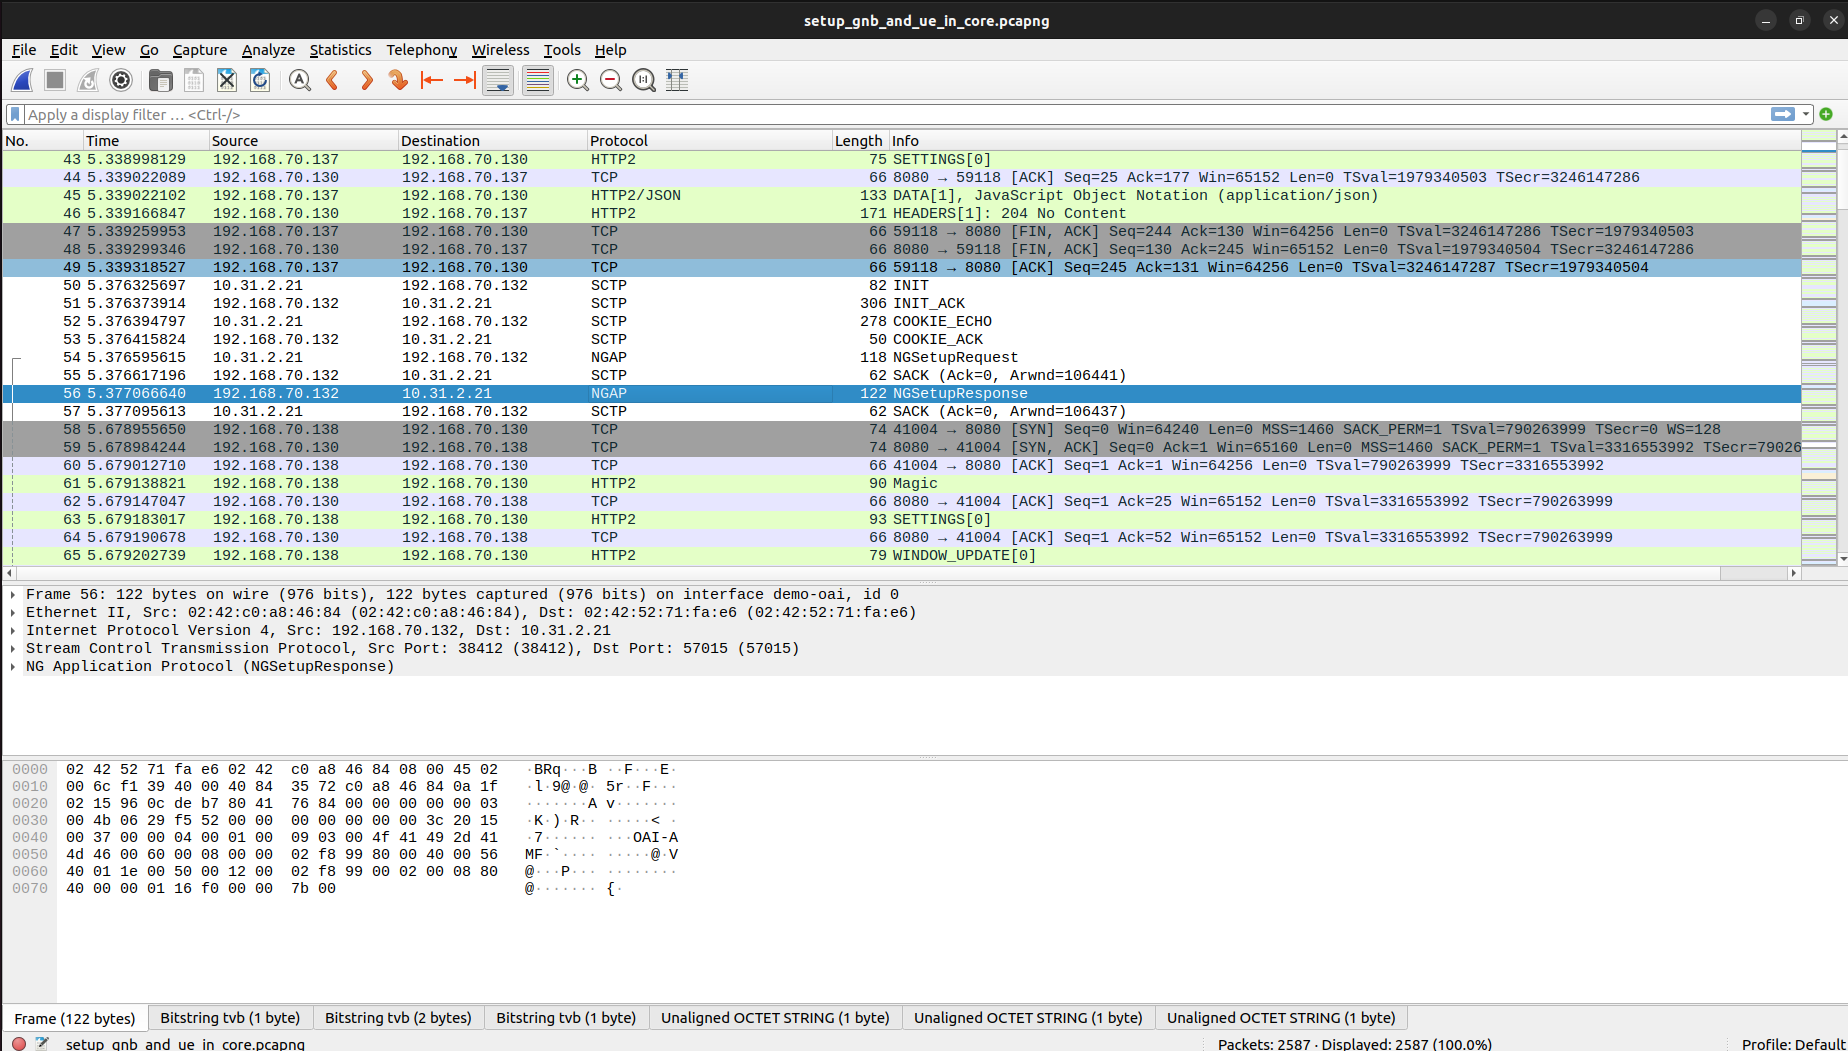
\includegraphics[width=0.8\linewidth]{figures/register_gnb}
    \caption[gNB registering via N2 interface]{gNB registering via N2 interface.}
    \label{fig:gnb_reg}
\end{figure}

The final verification was to check the connection between FlexRIC and gNB through the E2 interface.
This can be observed in the terminal running FlexRIC, where logs show the registration,  as depicted in Figure~\ref{fig:gnb_e2}.

\begin{figure}[H]
    \centering
    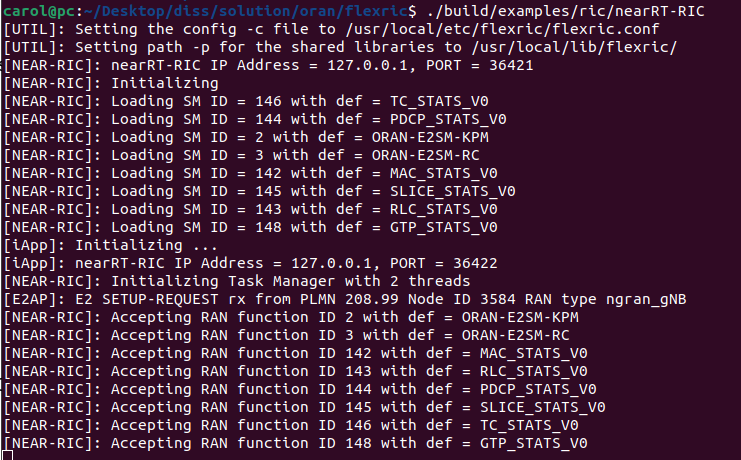
\includegraphics[width=0.5\linewidth]{figures/gnb_e2_flexric}
    \caption[gNB's E2 node registering with FlexRIC]{gNB's E2 node registering with FlexRIC.}
    \label{fig:gnb_e2}
\end{figure}

\subsection{UE}\label{subsec:ue}

In order to test the correct initialization of the UE, we needed to ensure connection with the Core Network.
After launching the UE, using the command present in~\ref{subsec:oai-5g-ue}, we observed the correct registration of the UE in Wireshark , as shown in Figure~\ref{fig:registration_ue}.

\begin{figure}[H]
    \centering
    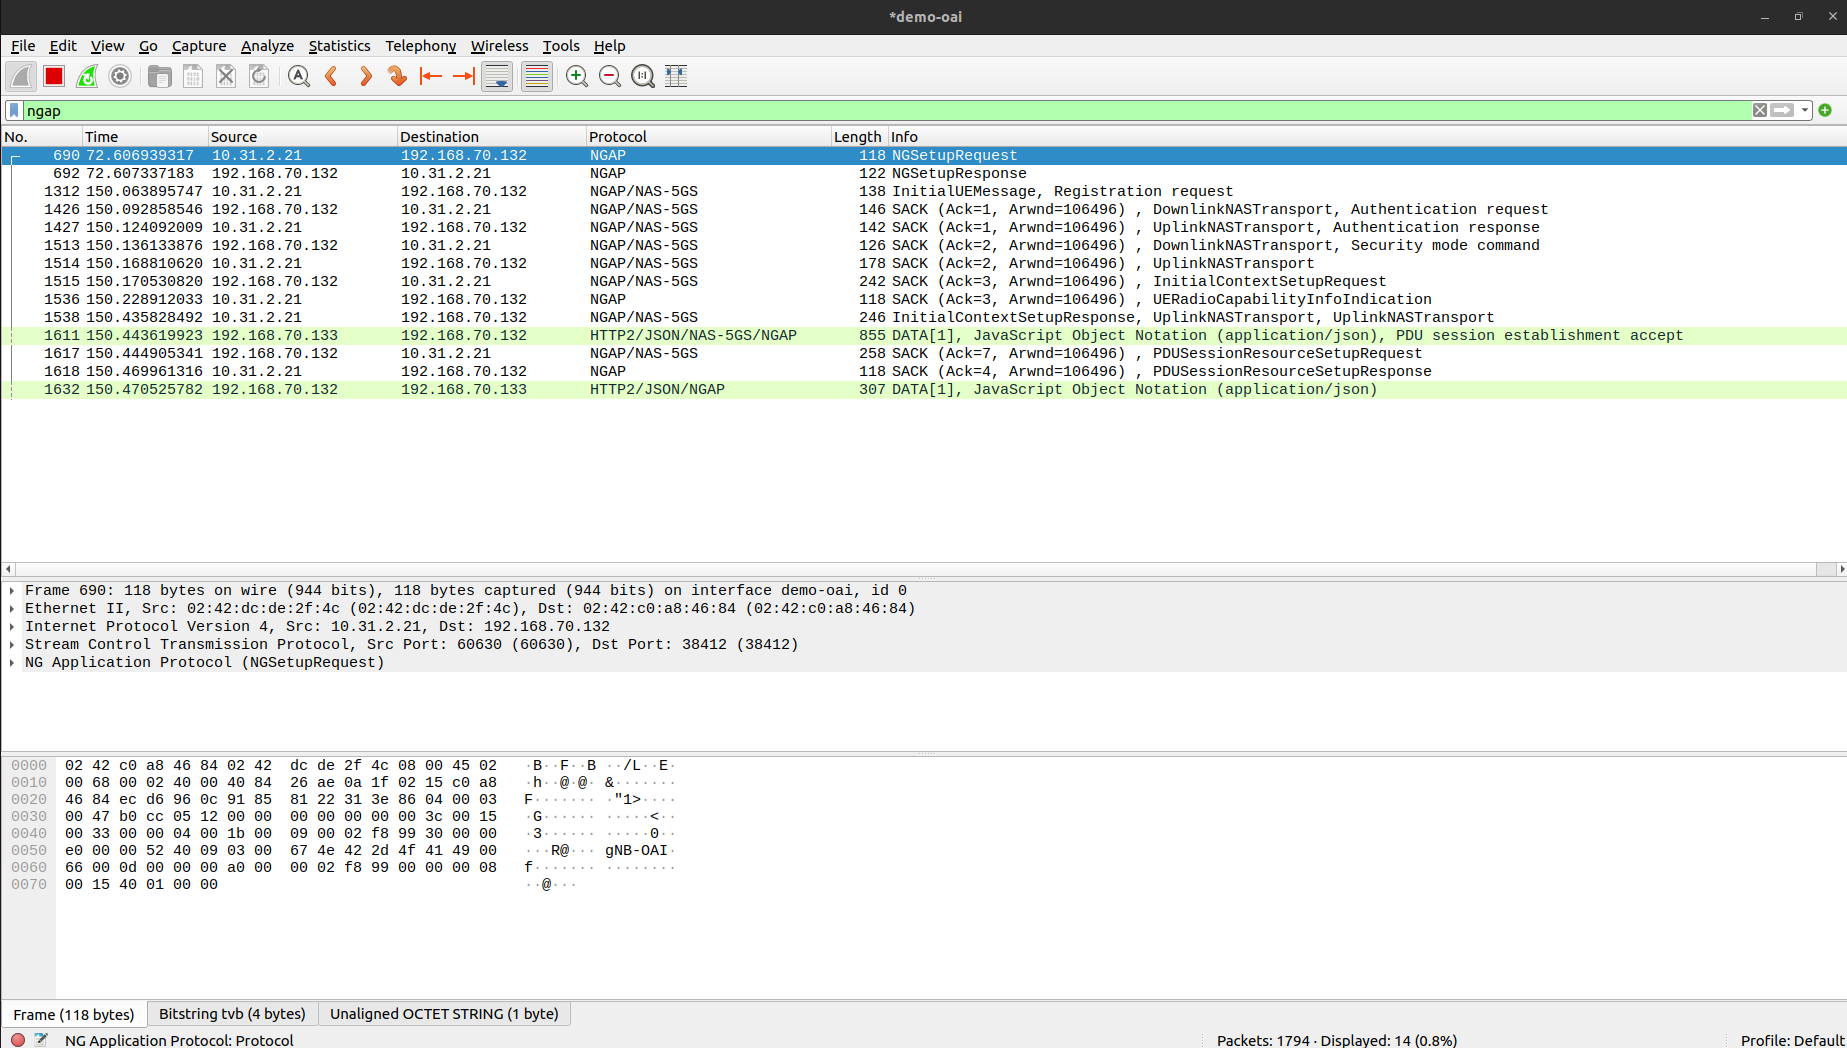
\includegraphics[width=0.8\linewidth]{figures/ue_registration}
    \caption{Registration of the UE.}
    \label{fig:registration_ue}
\end{figure}

When this synchronization occured, we verified the creation of \textit{oaitun\_ue1}, the tunnel interface between the UE and the Core Network.
After that, we assessed the connectivity, by pinging every Core Network component, as well as the Internet.
Figure~\ref{fig:ping_ue_core} and Figure~\ref{fig:ping_ue_internet} show the outcome of the connectivity tests to the Core Network and the Internet, respectively.

\begin{figure}[H]
    \centering
    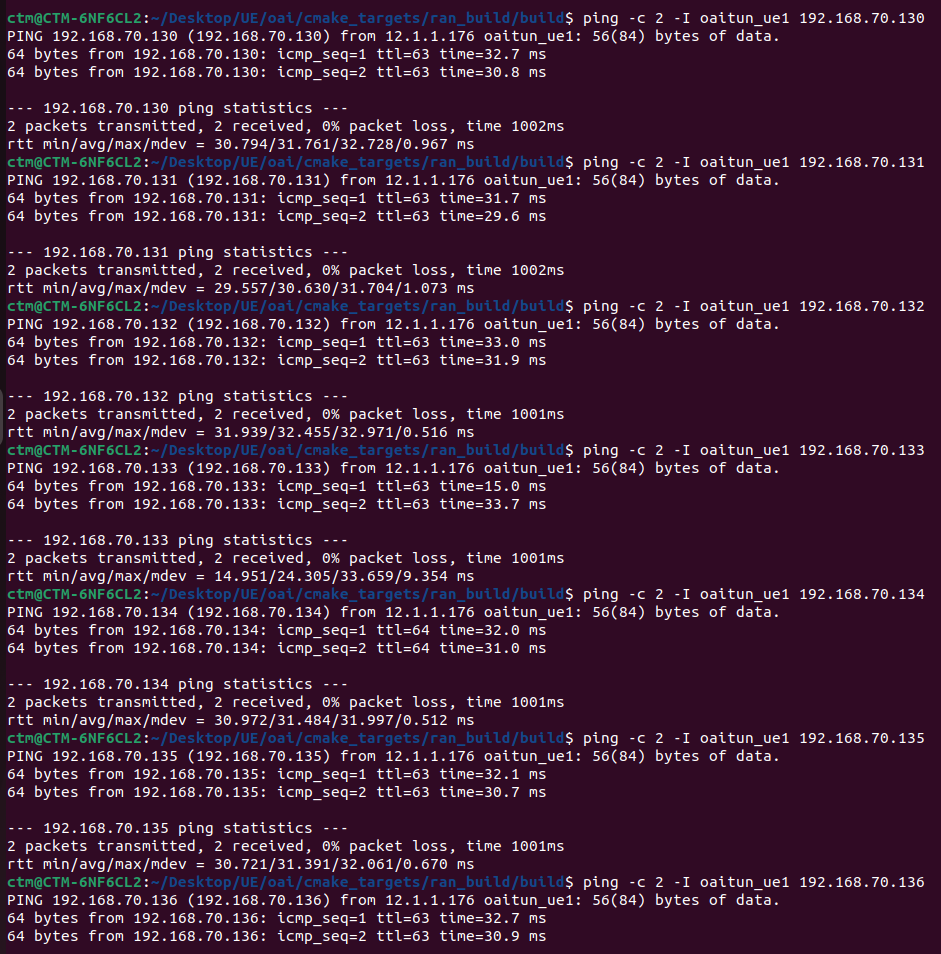
\includegraphics[width=0.5\linewidth]{figures/ue_core_ping}
    \caption{Pinging from UE to the Core Network components.}
    \label{fig:ping_ue_core}
\end{figure}

\begin{figure}[H]
    \centering
    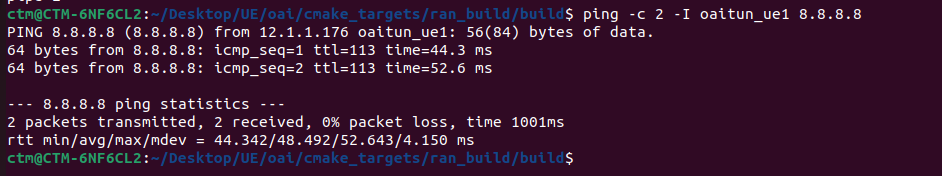
\includegraphics[width=0.5\linewidth]{figures/ue_to_ext}
    \caption{Pinging from UE to Google's public DNS server.}
    \label{fig:ping_ue_internet}
\end{figure}


\subsection{Vision Module}\label{subsec:cv_module}
To ensure the correctness and reliability of the VM, a series of validation tests was conducted.
These tests were designed to evaluate both the processing capabilities of the module and the accuracy of message exchange between the VM and the xApp.

The time for processing a frame varies according to several factors, such as the complexity (i.e.\ number of objects present) and the temporal variation of the scene.
This impacts in design choices such as the periodicity of metric extraction by the xApp.
The processing time for each frame was measured to assess the performance of the VM\@.
The average processing time when testing with real-time capturing is 5 frames/s\@.
While this is 17\% of the frame capture rate, it is sufficient to evaluate if our solution allows the adaptation of the gNB\@.

A reference video was used to evaluate the detection and tracking results of the VM\@.
This video, containing people walking, was processed to check detection accuracy and tracking consistency.
It was confirmed that the module could accurately detect and track objects, validating its effectiveness in real-world scenarios.
Figure~\ref{fig:reference_video} shows a capture of such the processed video.

% image of a frame of the video and the corresponding messages

\begin{figure}[H]
    \centering
    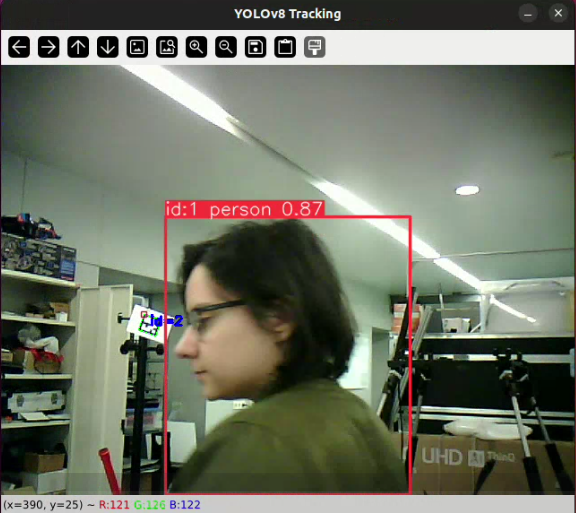
\includegraphics[width=0.7\linewidth]{figures/reference_frame}
    \caption{Reference post-processed video presenting an identified obstacle (person) and the ArUco marker representing the UE.}
    \label{fig:reference_video}
\end{figure}

Print statements were used on the server side to verify the correct formatting, encoding, and decoding of the messages.
This step was crucial to ensure that the messages sent from the module to the xApp were correctly structured and could be properly interpreted upon receipt.

On the client side, the xApp, print statements were employed to confirm the correct reception of the messages.
This validation step ensured that the messages transmitted through the socket connection were properly received and could be correctly processed.

To further validate the communications, Wireshark was used to capture SCTP packets containing the messages exchanged between the server and client, as shown in Figure~\ref{fig:capture_messages}.
This capture provided a view of the message flow, confirming that the messages were transmitted as expected without any loss or corruption.

\begin{figure}[H]
    \centering
    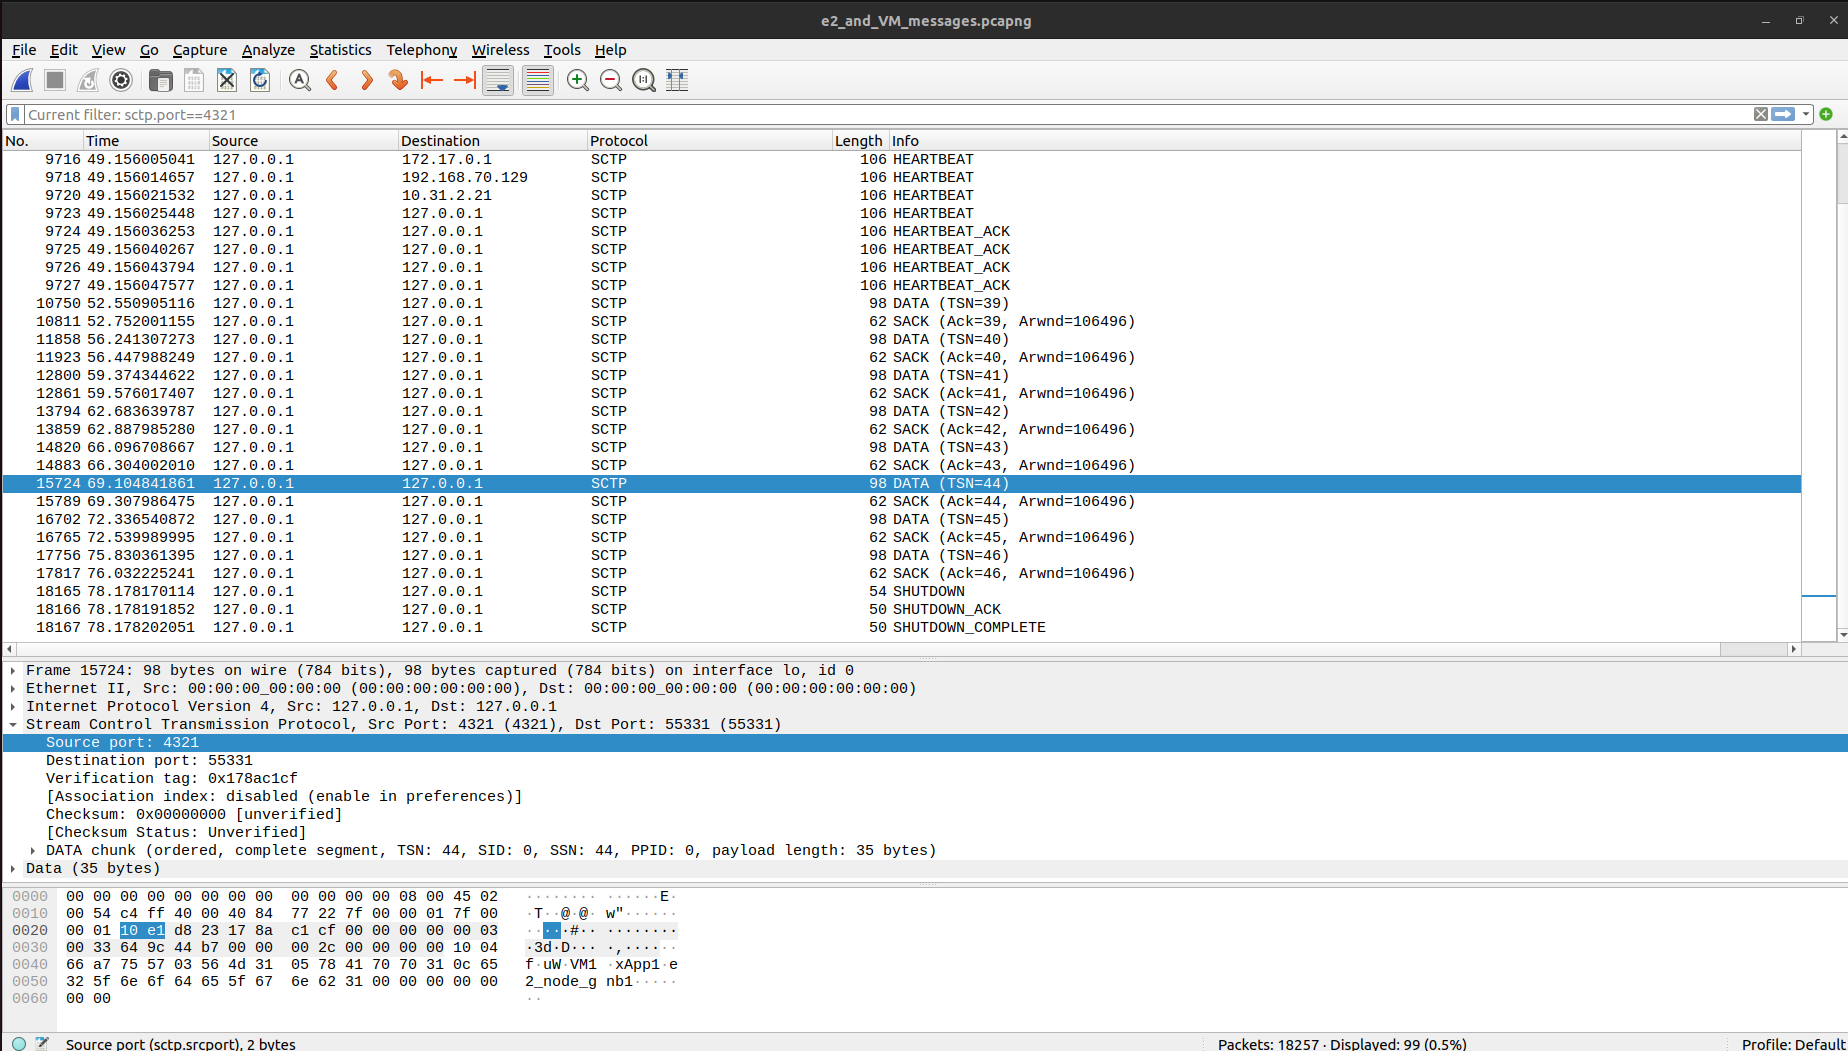
\includegraphics[width=0.8\linewidth]{figures/vm_xapp}
    \caption[SCTP packet exchange between VM and xApp]{SCTP packet exchange between VM and xApp.}
    \label{fig:capture_messages}
\end{figure}

The VM's performance proved adequate for the intended application, considering an indoor environment where movements are frequent yet the velocity is low, such as people walking or objects being moved.
The module demonstrated good performance in these scenarios, and its near-real-time processing capability can trigger prompt reactions to environmental changes.

\subsection{xApp}\label{subsec:mm_xapp}
After all components of our system were deployed and properly functioning, we assessed the correct functioning of the xApp.
The first verification was to check if the xApp could communicate with the FlexRIC software.
This allows the E2 subscription to the E2 node on the gNB, to retrieve data from it.
Figure~\ref{fig:xapp_subscription} shows this process.

\begin{figure}[H]
    \centering
    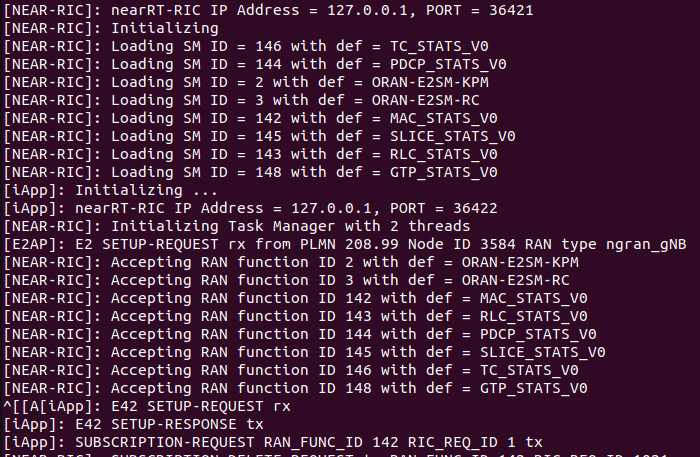
\includegraphics[width=0.5\linewidth]{figures/xapp_subscription}
    \caption{FlexRIC receiving the subscription request from the xApp.}
    \label{fig:xapp_subscription}
\end{figure}

E2 indication messages were received by the xApp once the subscription process was concluded.
The periodicity of these messages can be defined in the xApp.
We chose to receive MAC layer metrics every 10 ms to obtain SNR measurements.
These values are essential for the state machine described in Section~\ref{subsec:xapp}.
The E2 subscription procedure can be seen in Figure~\ref{fig:captura_e2ap}.

\begin{figure}[H]
    \centering
    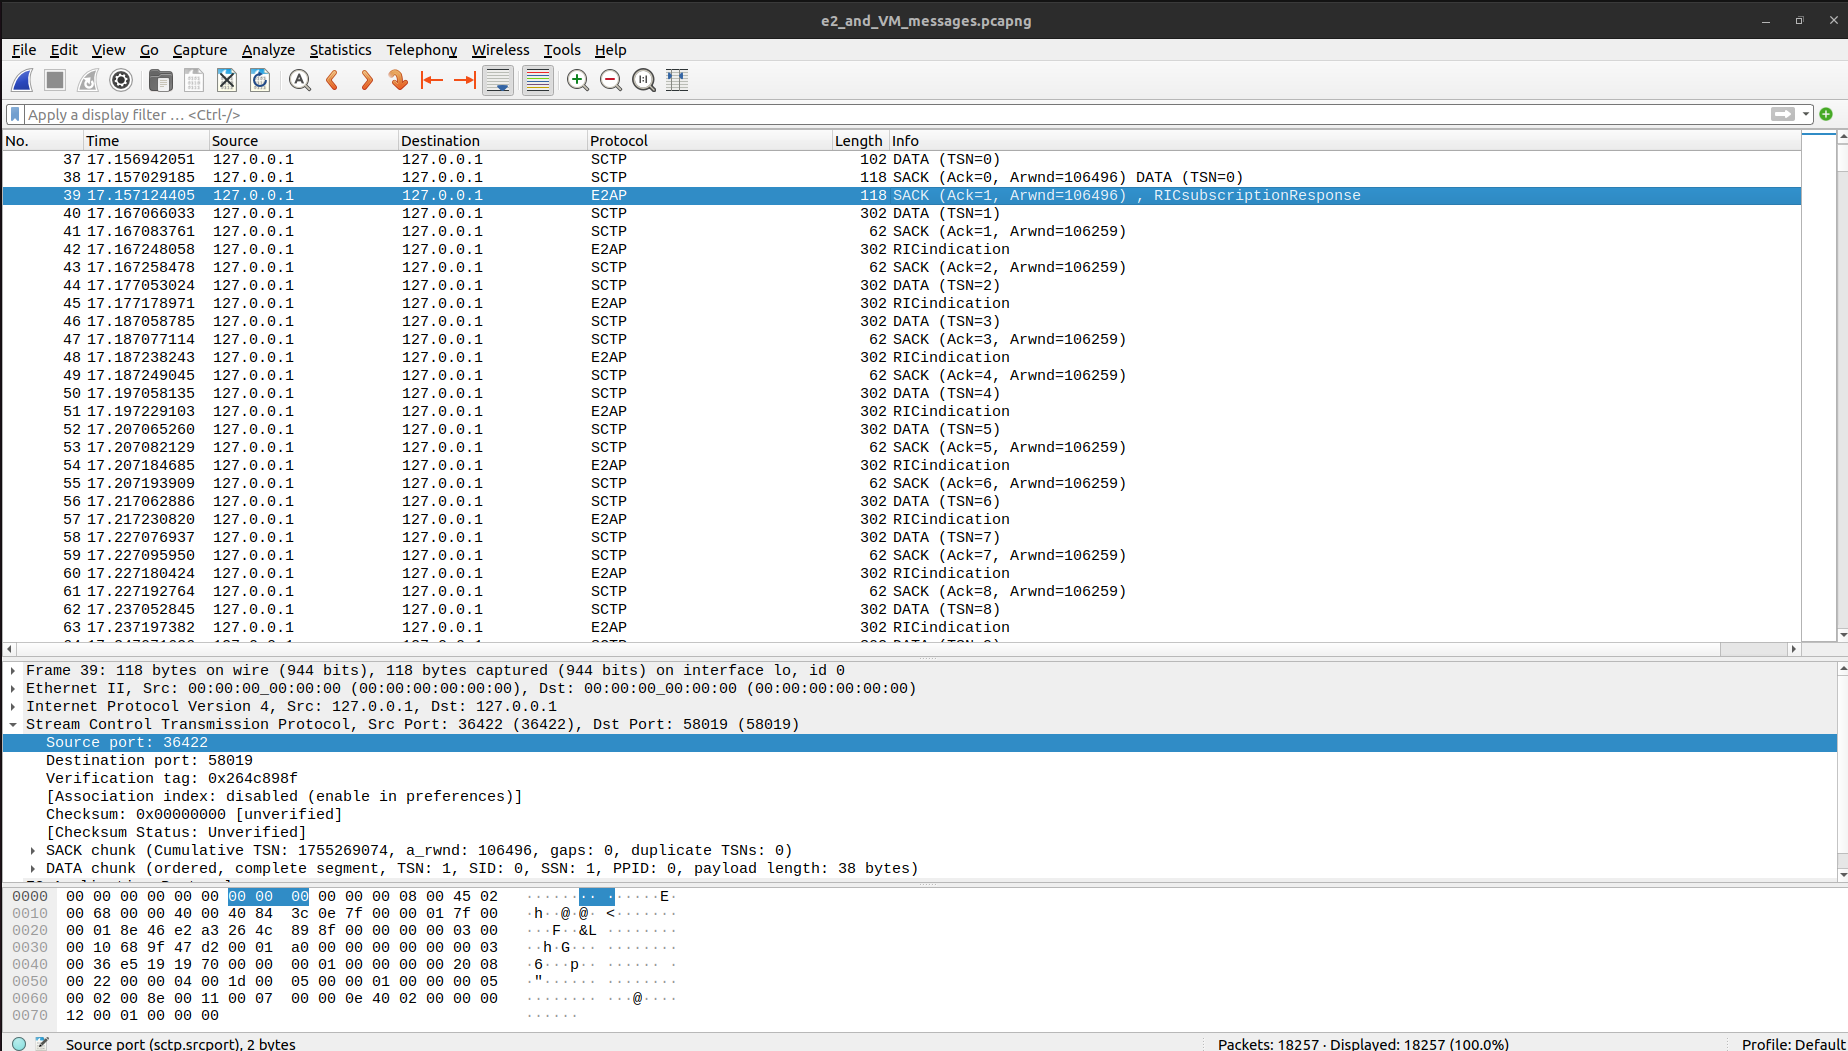
\includegraphics[width=0.8\linewidth]{figures/ric_subs}
    \caption{E2 Subscription Response and E2 Indication messages.}
    \label{fig:captura_e2ap}
\end{figure}

\section{Use case}\label{sec:use_case}
In order to validate the implemented solution, a use case testing scenario was defined.
In an indoor environment, the system considered the architecture presented in Figure~\ref{fig:my_arch}.
The figure showed the vision-aided RAN, comprising the gNB and the VM, and their connections with the near-RT RIC, the xApp, the UE and 5G Core Network.

The goal of test was to assess the functionality of the whole system, considering maintaining channel quality, or increasing it whenever possible.
The xApp suggests repositioning the gNB, based on data collected from the Vision Module and the RF metrics collected from the RAN via the Near-RT RIC\@.

The use case demonstrates the system's capabilities in four test scenarios, described in the following subsections.
For all scenarios we assume a constant velocity for all moving entities.

\subsection{Scenario A : Fixed gNB and UE}\label{subsec:scenario-0-:-fixed-gnb-and-ue}

In this scenario, the objective was to assess the impact of blockages on the LoS between the gNB and the UE\@.
By maintaining a fixed position for both the gNB and the UE, we could introduce obstacles to observe their effects on signal quality.
This scenario also aimed at validating the accuracy of the messages sent by the VM regarding the presence of blockages.
Figure~\ref{fig:test_fixed} depicts a top-view from the testing scenario.
This scenario contain two variations: one where the obstacle moves at a constant velocity and one where the obstacle holds its position for a few seconds.

\subsubsection{Constant velocity}
The obstacle moves from left to right, over time at a constant velocity.

The results from this scenario serve as a baseline for comparison with other scenarios, in which the positions of the gNB and UE may vary.
This analysis is important for evaluating the benefits of integrating CV solutions into mobile networks.

\begin{figure}[H]
    \centering
    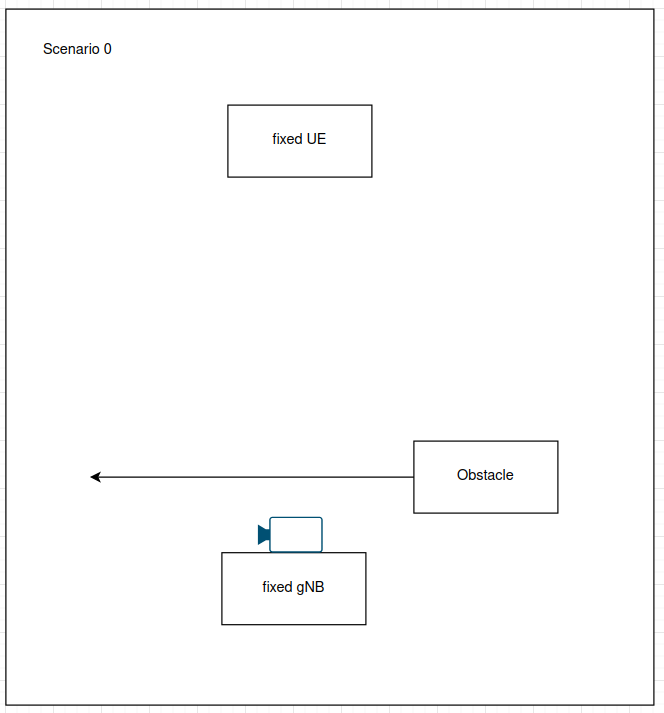
\includegraphics[width=0.5\linewidth]{figures/scenario0}
    \caption{Overview of the movement for scenario A.}
    \label{fig:test_fixed}
\end{figure}

\begin{figure}[H]
    \centering
    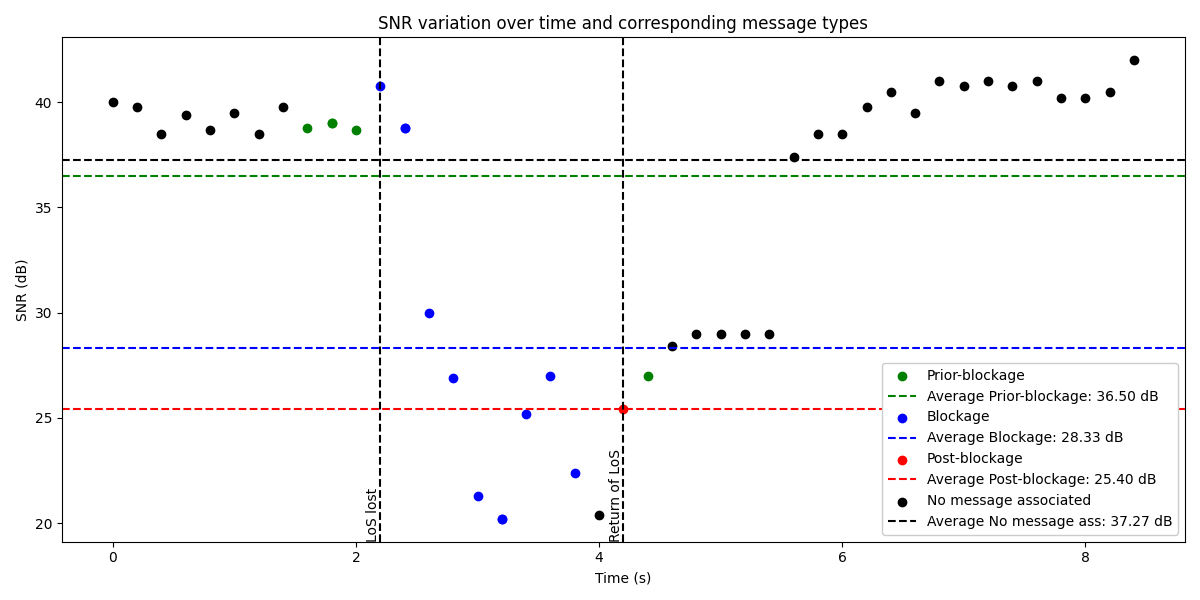
\includegraphics[width=\linewidth]{figures/results_0}
    \caption{SNR variation over time and the respective VM messages for scenario A at constant velocity.}
    \label{fig:results_0}
\end{figure}


This test was successful, showcasing the CV module messages received, as well as SNR metrics corresponding to those expected.

Figure~\ref{fig:results_0} presents a graph with the results collected from this experiment.
The to see the SNR variation over time is shown on in the y-axis, associated with each message.
The average SNR values are collected by the xApp in intervals of 200 milliseconds (20 samples collected periodically every 10 ms).
Possible intervals for this data collection are 1 ms, 2 ms, 5 ms, or 10 ms.
This value is set according to the estimated processing framerate of the video.
Since prior tests have shown that capturing at 30 frames/s results in the processing of video at about 5 frames/s, we chose this value so that each message reception has an SNR value associated.
Each message is represented by a color, as shown in the legend.
Note that we can also have situations were there are SNR values but no associated message, for instance when the detected obstacles are not expected to block the LoS\@.

The graph is divided into three distinct stages, separated by transition lines.
In the first stage, where the obstacle is moving towards the UE, Prior Blockage messages are sent.
The SNR is high  since there is no obstruction of LoS between gNB and UE, indicating a strong signal.

The first transition is labeled \('\)LoS lost\('\), marking the beginning of the blockage period.
It is important to note that since the ArUco is positioned to the left of the SDR, the blockage from the CV perspective happens first and then the LoS, from the radio perspective, is lost.
This explains why the SNR only lowers after a few Blockage messages.

In the second stage,the obstacle stops in front of the UE and the reception of the first Blockage Message is observed, indicating the beginning of the obstruction.
As expected, the average SNR decreases.

The second transition is labeled \('\)Return of LoS\('\), indicating the end of the blockage and the return to normal signal conditions.
In the third stage, the obstacle moves away from the UE, no longer blocking the LoS\@.
As expected, the average SNR approximates those seen in the first stage.
The SNR values increase, similar to the prior blockage stage, indicating the restoration of a strong signal, suggesting the passage of the blockage.

In this scenario, we also used the iperf tool to test the throughput at two points.
The first was when no blockage was occurring.
The second was during a blockage.
This test considered TCP traffic and assessed the uplink throughput.
As expected, the throughput was lower during a blockage.
Table~\ref{tab:iperf} presents the measured values.


\begin{table}[h]
    \centering % Center the table
    \begin{tabular}{|c|c|c|c|}
        \hline
        \textbf{Instant} & \textbf{Throughput} \\ \hline
        No blockage & 7.67 Mbits/s \\ \hline
        Blockage   &  5.27 Mbits/s \\ \hline
    \end{tabular}
    \caption{Throughput results for LoS and NLoS.} % Add a caption for the table
    \label{tab:iperf} % Add a label for referencing the table
\end{table}

\subsubsection{Holding position}

The obstacle moves from left to right.
It first holds its position in the camera field of view, without blocking the LoS\@.
After a few seconds it moves to a blocking position and holds still for a few seconds.
Finally, it leaves the blocking position.

The test was successful.
Figure~\ref{fig:results_01} presents a graph with the results collected from this experiment.
This graph is similar to the one presented by Figure~\ref{fig:results_0}, as expected.

It is noticeable that the SNR between the blocked and unblocked states is more pronounced than in the scenario where the obstacle moves continuously.

This results in a more uniform distribution of SNR values associated with each message.
The SNR variation is more coherent with the messages.
For instance, the average SNR values for blockage messages is much lower than in the previous experiment, since the communications suffer attenuation for a longer period.


\begin{figure}[H]
    \centering
    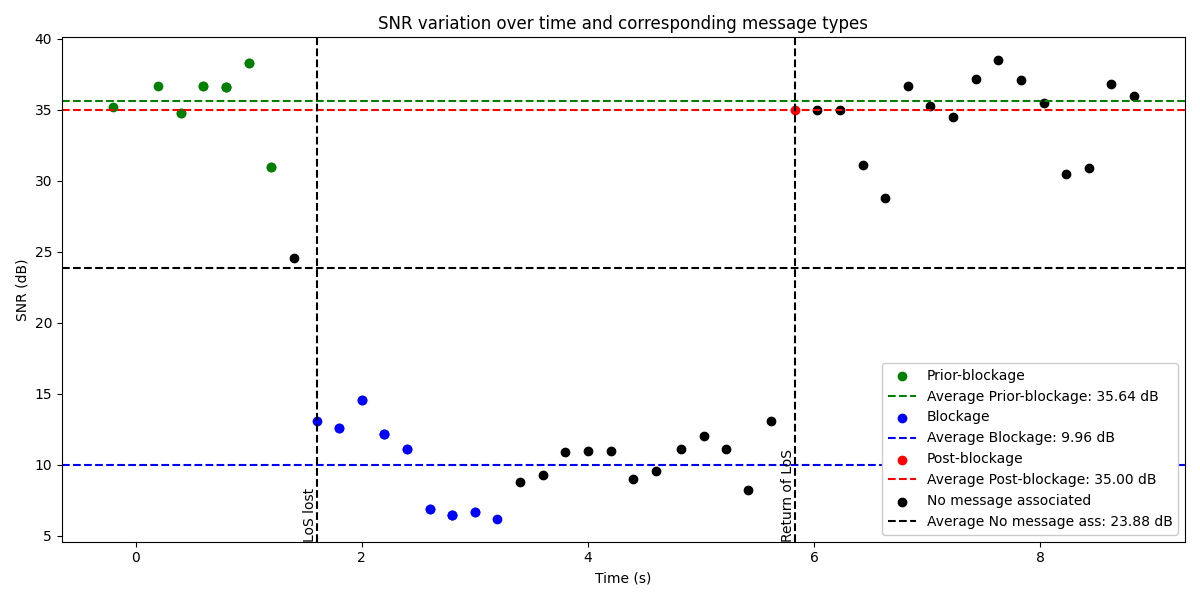
\includegraphics[width=\linewidth]{figures/results_01}
    \caption{SNR variation over time and the respective VM messages for scenario A, while holding the obstacle holds the position.}
    \label{fig:results_01}
\end{figure}


\subsection{Scenario B: Fixed gNB, moving UE}\label{subsec:scenario-0.1:-fixed-gnb-moving-ue}

In this scenario, the objective was to assess the limitations of our VM and characterize the occurrence of messages, including how the vision-aided gNB behaves when there is a moving UE\@.
The UE was carried by a person and the VM model could detect both the person and the UE\@.
Figure~\ref{fig:test_movUE} presents a top-view of the testing scenario.
The UE moved away from the gnB, at a constant velocity.
It stops briefly and rotates left slowly.
This movement is important to characterize to interpret the results of the graph.

\begin{figure}[H]
    \centering
    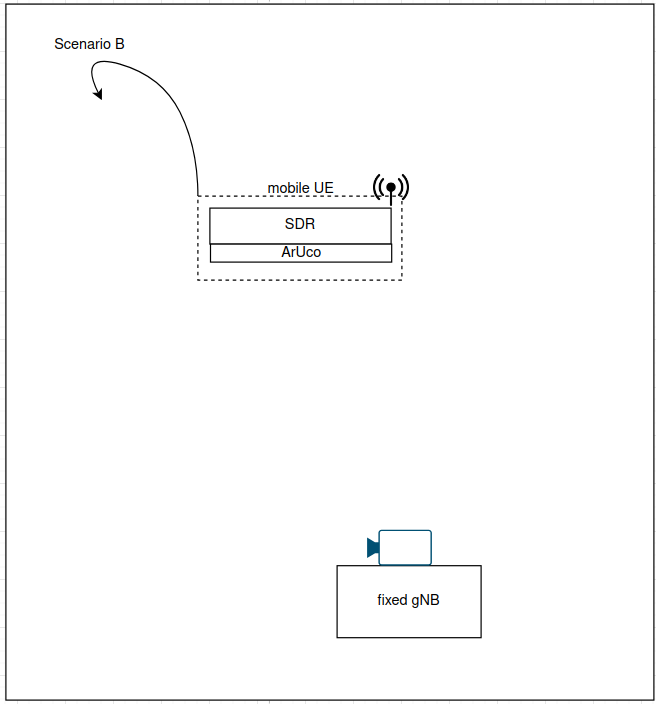
\includegraphics[width=0.5\linewidth]{figures/scenario1}
    \caption{Overview of the movement for scenario B.}
    \label{fig:test_movUE}
\end{figure}

This test occurred as expected.
We noticed that the VM generated incorrect messages, especially regarding Prior Blockage message, as anticipated.
This is because the module has no notion of depth.
It interprets the person as an obstacle and calculates that the bounding box movement of the person will intersect with the UE's.

Despite this limitation, it is evident that the VM does not emit Blockage messages, since the UE has LoS with the gNB\@.
Similarly, it does not emit Post Blockage messages.
Nonetheless, the system does support the movement of the UE, as at each frame, it checks the current position of the marker.

Figure~\ref{fig:results_1} presents a graph with the results collected from this experiment.
Some Prior Blockage messages are associated with these SNRs, while no obstacle is expected to block the LoS\@.
The VM module sends these messages because it viewed the person carrying the UE as an obstacle, and the person was moving in the same direction as the UE\@.
The SNR variation is shown in the y-axis, associated with each message.
Note that there is a variation in the SNR as the distance between the gNB and UE increased.
The period with no messages associated (black dots) corresponds to the period the UE was static.
Since the person carrying it was not moving, there were no obstacles moving towards the UE, in the perspective of the VM\@.
As UE rotated, the person was moving again, returning to the indication of Prior Blockage messages.
The rotation of the UE causes a variation on the SNR\@.
As the UE's antennas rotate closer to the gNB, the SNR increases.

\begin{figure}[H]
    \centering
    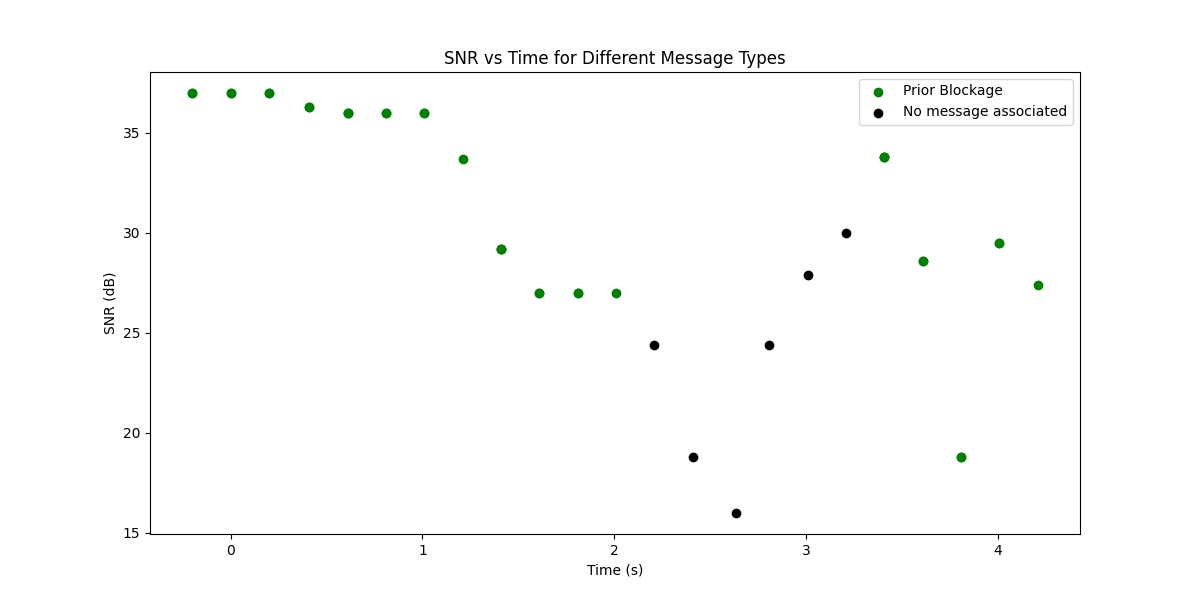
\includegraphics[width=\linewidth]{figures/results_1}
    \caption{SNR variation over time and the respective VM messages for scenario B.}
    \label{fig:results_1}
\end{figure}

\subsection{Scenario C: Fixed gNB, moving UE, Obstacle present}\label{subsec:scenario-0.1:-fixed-gnb-moving-ue-obstacle-present}

In this scenario, the objective was similar to the previous, we aimed at assessing how the vision-aided gNB behaves when there is a moving UE and multiple objects in the scene (a person carrying the UE and an obstacle represented by another moving person)\@.
The UE was carried by a person and the VM model could detect both the people and the UE\@.
Figure~\ref{fig:test_movUE} depicts a top-view of the testing scenario.
Although a person was carrying the UE, its position only residually changed, while the obstacle moved from left to right.

\begin{figure}[H]
    \centering
    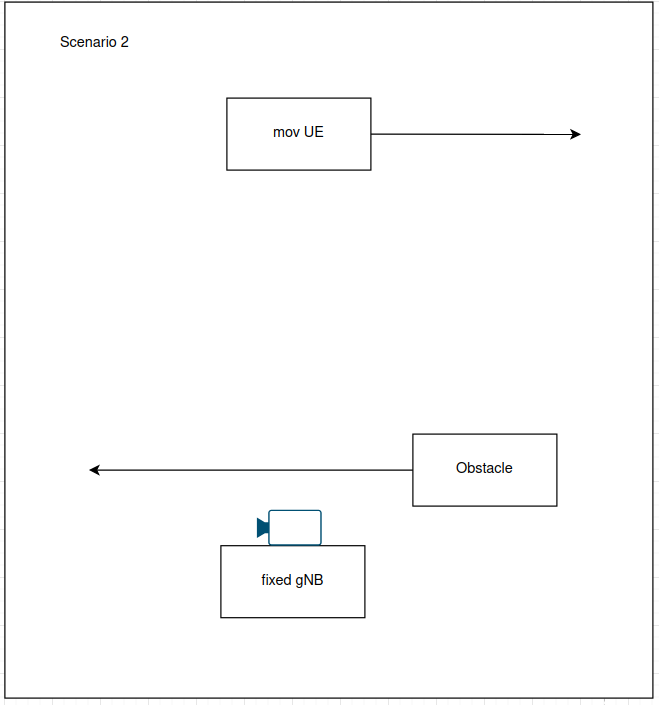
\includegraphics[width=0.5\linewidth]{figures/scenario2}
    \caption{Overview of the movement for scenario C.}
    \label{fig:test_movUE_obst}
\end{figure}

This test proceeded as expected.
Similar to the previous scenario, the VM generated incorrect messages, especially when it came to Prior Blockage messages, as anticipated.
The difference from the previous scenario is that the VM still generated correct messages concerning the obstacle in the foreground of the frame.

Figure~\ref{fig:results_2} presents a graph with the results collected from this experiment.
The SNR variation over time can be seen in the y-axis, associated with each message.
In the graph, the first Blockage messages happened before the obstruction of the LoS\@.
The reason is that the ArUco is positioned to the left of the antenna, similarly to scenario A\@.
This means that a few of these messages are received before the LoS is blocked and consequently, the SNR drastically decreases.

The positioning of the video camera too close to the objets is one of the reasons this happens.
When a camera is close to the objects, they are perceived bigger and limiting the field of view.
In our case, this means that both in the Blockage messages and the Post Blockage message, the LoS is not completely synchronized with the messages.
This limitation is caused by the short range of the SDRs, making it difficult to have 2 people and use the absorbing material in a range of 2 m.

One relevant note is the no message associated in this scenario.
This happened because this corresponded to a moment were no detections were made by YOLO, since the RF absorbing material was covering the camera's field of view and the model is not trained to recognize such class of object.
Hence, no detection of obstacle or marker was made during this period, and no messages generated by the VM\@.
It is specially relevant to mention this as it indicates our system can accurately detect objects and in other scenarios would not assume any object is an obstacle, since we only selected from the classes available those relevant from the RF perspective.

\begin{figure}[H]
    \centering
    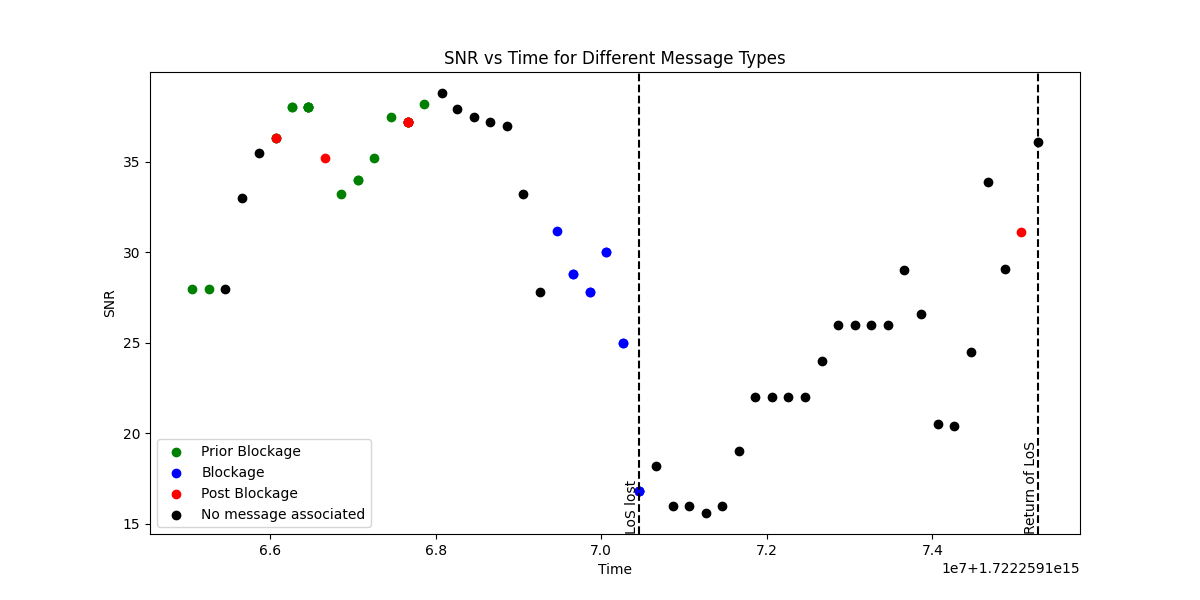
\includegraphics[width=\linewidth]{figures/results_2}
    \caption{SNR variation over time and the respective VM messages for scenario C.}
    \label{fig:results_2}
\end{figure}

\subsection{Scenario D: Moving gNB}\label{subsec:scenario-3:-moving-gnb}

In this scenario, the objective was to move the gNB to maintain LoS\@.
We assessed the vision-aided gNB predictions and evaluated the benefits of moving a gNB\@.
The gNB was moved on a table and the VM model could detect the obstacle and the UE\@.
Figure~\ref{fig:test_movgnb} shows a top-view of the testing scenario.
The UE was fixed, the obstacle moved from right to left at constant pace, and the gNB moved in the opposite direction.

\begin{figure}[H]
    \centering
    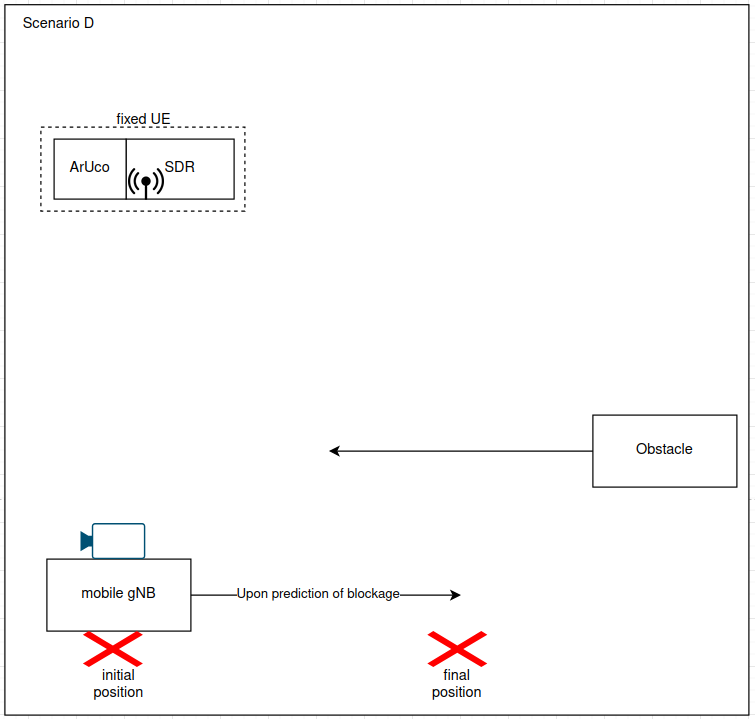
\includegraphics[width=0.5\linewidth]{figures/scenario3}
    \caption{Overview of the movement for scenario D.}
    \label{fig:test_movgnb}
\end{figure}

Figure~\ref{fig:results_3} depicts a graph with the results collected from this experiment.
The SNR variation over time on the y-axis, associated with each message.

One noticeable factor is that we could not preventivelly move the gNB due to human time reaction, leading to a blockage.
We needed to read a Prior Blockage message and reposition the gNB before the obstacle (person walking) reached the UE\@.
Although we could not do this before the break of LoS, it returned after the repositioning of the gNB\@.

Despite this setback on the movement of the gNB, we could obtain data and valuable information regarding the experiment.

\begin{figure}[H]
    \centering
    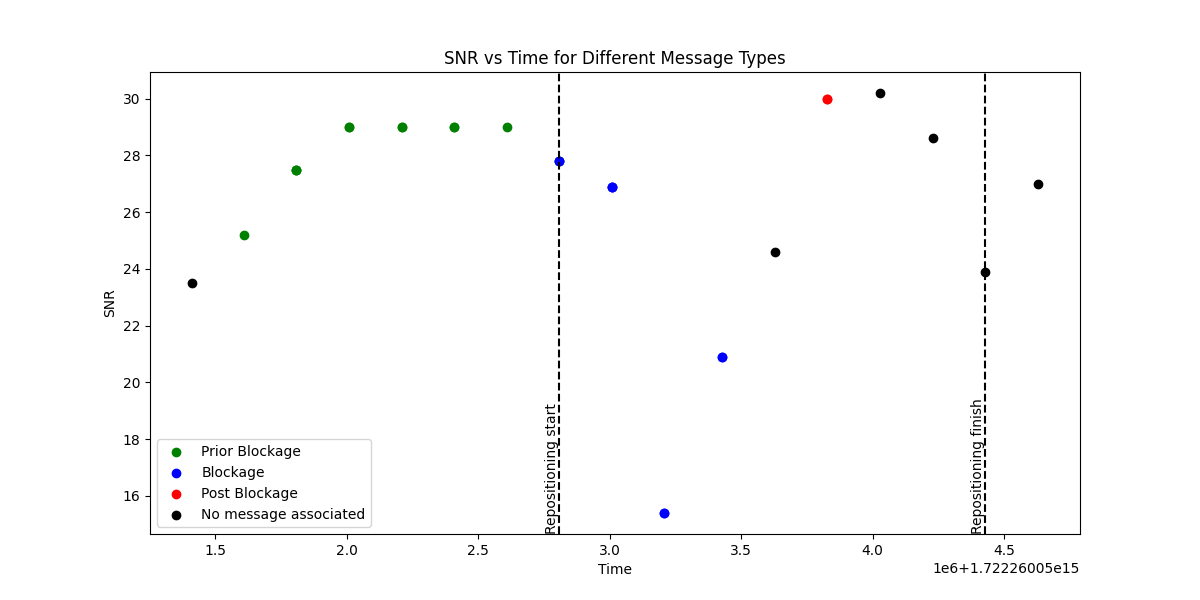
\includegraphics[width=\linewidth]{figures/results_3}
    \caption{SNR variation over time and the respective VM messages for scenario D.}
    \label{fig:results_3}
\end{figure}

In the graph, there are two transition moments.
The first is represented by \('\)Repositioning start\('\), indicating the moment the Prior Blockage message are perceived and the movement of the gNB started.
As expected, the SNR lowers when the Blockage happens.
In this scenario, the LoS is recovered faster than in scenario A, since repositioning the gNB enables it.

The second transition \('\)Repositioning finish\('\) indicates the moment the repositioning of the gNB ends.
The reposition ends after LoS is recovered and, as expected, the average SNR increases, reaching similar values to the prior blockage stage, indicating the restoration of a strong signal, suggesting the passage of the blockage.
After the Post blockage message, no obstacles are estimated to block the LoS and the VM does not send messages.

%\subsection{Scenario 2: UE Moving Away from the gNB}\label{subsec:scenario-2:-ue-moving-away-from-the-gnb}

%This scenario involves the UE moving progressively further from the gNB. In the absence of identified obstacles, a decrease in the Signal-to-Noise Ratio (SNR) is interpreted as the UE increasing its distance from the gNB. To address this, the robotic platform, leveraging the Mobility Management xApp, dynamically moves towards the UE to uphold optimal communication quality.
%This adaptive response ensures that the UE remains within the effective communication range of the gNB, thereby maintaining robust and reliable connectivity.


\section{Discussion}\label{sec:discuss}
The tests validated the proposed solution, demonstrating that the objectives of this dissertation were achieved.
Component tests confirmed the operational status of all individual entities, ensuring that each part of the system functioned correctly.
Interoperability tests verified the integration of these entities, confirming that the system operated cohesively as a whole.
The evaluation demonstrated the viability of the proposed solution, indicating its potential for application in real-world scenarios.

In terms of the data extracted form the video, we noticed the correct generation of Blockage Messages and Post Blockage messages.
Prior blockage messages are generated frequently and in some cases, incorrectly.
For this message type, we intentionally opted for detecting more false positives than false negatives in order to avoid ignoring a real potential blockage.
Since the RAN is responsible for the placement management, having more false positives messages is not critical in the VM\@.

Our solution enables the RAN to assess if the variation of the SNR is caused by an obstruction in LoS\@.
The SNR variations were complemented by the CV data, providing reliable information to the RAN\@.
Our solution can detect several types of obstacles, such as people, furniture, and pets in indoor scenarios, providing information such as the velocity of the obstacle, the time to expect the blockage.
One important limitation to mention is the fact that currently it only supports one UE\@.

Despite limited testing conditions, it was possible to identify the functionality, capabilities and limitations of the system, and specially the VM\@.
We could validate that the system can be implemented to maintain LoS in specific contexts, in which the video camera has a good field of view of the scene.
The inclusion of an automatic repositioning within the xApp may also benefit this solution.

The use of O-RAN facilitated the introduction of technologies within the RAN\@.
Specifically, the use of an xApp to incorporate CV messages, enhanced RAN capabilities.
This integration showcased the flexibility and potential of O-RAN in enabling solutions that improve wireless networks.

